%-------------------------------------------------------------------------------
% LATEX TEMPLATE ARTIKEL

%	PACKAGES EN DOCUMENT CONFIGURATIE
%-------------------------------------------------------------------------------

\documentclass{uva-inf-article}
\usepackage[english]{babel}
\usepackage{graphicx}
\usepackage{tikz}
\usetikzlibrary{decorations.pathreplacing, angles,quotes}
\usepackage{amsmath}
\usepackage{amssymb}
\usepackage[title]{appendix}
\usepackage{lscape}
\usepackage{booktabs}
\usepackage{mathtools} % \shortintertext{}
\usepackage{physics}
%Theoremstyle etc. 
\usepackage{amsthm}
\addtolength{\jot}{8pt} % Extra spacing for equations
% Define new theorem "Definition" 
\theoremstyle{definition}
\newtheorem{definition}{Definition}[section]
\newtheorem{corollary}{Corollary}
% Multicolumn environment 
\usepackage{multicol}
% position pictures in text
\usepackage{float}
% line break in table cells
\usepackage{makecell}
% Color table cells
\usepackage{xcolor, colortbl}
% number equations within one section 
\numberwithin{equation}{section}
% Format picture captions
\usepackage[margin={-30pt,20pt}, indention= 2em, font=small,labelfont=bf, labelsep=period]{caption}
%\usepackage{caption}
\usepackage{subcaption}
% Redefine Figure in Multicol 
\newenvironment{Figure}
  {\par\medskip\noindent\minipage{\linewidth}}
  {\endminipage\par\medskip}
%Algorithms
\usepackage{algorithm}
\usepackage[noend]{algpseudocode} % omit if-end, for-end aso

\usepackage[style=ieee]{biblatex}
\addbibresource{references.bib}

\allowdisplaybreaks

\usepackage{framed}


%-------------------------------------------------------------------------------
%	GEGEVENS VOOR IN DE TITEL, HEADER EN FOOTER
%-------------------------------------------------------------------------------

% Geef je artikel een logische titel die de inhoud dekt.
\title{Research  notes}

% Vul de naam van de opdracht in zoals gegeven door de docent en het type 
% opdracht, bijvoorbeeld 'technisch rapport' of 'essay'.
\assignment{}
\assignmenttype{}

% Vul de volledige namen van alle auteurs in en de corresponderende UvAnetID's.
\authors{Aaron De Clercq\\aaron.de.clercq@student.uva.nl}
\uvanetids{14483610}



% Dit is de datum die op het document komt te staan. Standaard is dat vandaag.
\date{\today}

%-------------------------------------------------------------------------------
%	VOORPAGINA 
%-------------------------------------------------------------------------------

\begin{document}
\maketitle
%-------------------------------------------------------------------------------
%	INHOUDSOPGAVE EN ABSTRACT
%-------------------------------------------------------------------------------
% Niet toevoegen bij een kort artikel, zeg minder dan 10 pagina's!

%TC:ignore
\tableofcontents
\newpage
%\begin{abstract}
%\end{abstract}
%TC:endignore

%-------------------------------------------------------------------------------
%	INHOUD
%-------------------------------------------------------------------------------
% Hanteer bij benadering IMRAD: Introduction, Method, Results, Discussion.
\justifying

% Theory section
\section{Theoretical background}

This section covers the theoretical concepts necessary to understand the research project.

\subsection{Spin models}

One approach to represent a system is through a spin model. Assume a given system with $n$ components where a single observation of the system yields one value for every component.
Such an observation can be seen as a specific state of the system.

\subsubsection{Binary spin operators}

In case that the observations can be binarized, the state of the system can be written as a spin configuration,

\begin{equation}
    \mathbf{s} = (s_1 \dots s_n),
\end{equation}

\noindent
of $n$ spin variables, where every variable takes a value of either +1 or -1.

\noindent
In a spin configuration, we can express an interaction between a subset $\mu$ of these spins using a spin operator which is defined as the product of all spins in the subset,

\begin{equation}\label{eq:spin_op}
    \phi^\mu(\mathbf{s}) = \prod_{i \in \mu} s_i.
\end{equation}

\noindent
Given that all spin values are either +1 or -1, the spin operator will be +1 if an even number of spins are -1 and it will be -1 if an odd number of spins are -1.
The sum over all possible spin configurations of a spin operator is equal to zero,

\begin{equation}\label{eq:sum_over_conf}
    \sum_{\mathbf{s} \in \mathbf{S}} \phi^\mu(\mathbf{s}) = 0,
\end{equation}

\noindent
because half of the spin configurations can be written as a spin configuration in the other half with exactly one spinflip.
In a system with $n$ spin variables, there are $2^n - 1$ possible subsets, which means that there are $2^n - 1$ different spin operators.

\begin{definition}
    A set of operators, $\Omega$ is called orthogonal if

    \begin{equation}\label{eq:ortho}
        \frac{1}{2^n} \sum_{\mathbf{s} \in \mathbf{S}} \phi^\mu(\mathbf{s}) \phi^\nu(\mathbf{s}) = \delta_{\mu\nu} \qquad \forall \;\; \phi^\mu, \phi^\nu \in \Omega
    \end{equation}
\end{definition}

\begin{definition}
    A set of operators, $\Omega$ is called complete if

    \begin{equation}\label{eq:complete}
        \frac{1}{2^n} \sum_{\mu \in \Omega} \phi^\mu(\mathbf{s}) \phi^\mu(\mathbf{s}^\prime) = \delta_{\mathbf{s}\mathbf{s}^\prime},
    \end{equation}
    as this yields a unique relation between the spin configuration and the values for every operator in the set.
\end{definition}

\noindent
If we define the identity operator, $\phi^0 = 1$, then the set of operators $\Omega_n = \{\phi^\mu(\mathbf{s})\}_{\mu \in \{0 \dots 2^n-1\}}$ is a complete and orthogonal set.
For orthogonality, we can rewrite Equation \ref{eq:ortho}, use Equation \ref{eq:sum_over_conf} if $\mu$ and $\nu$ are different and use the definition of the identity operator if $\mu$ and $\nu$ are the same.

\begin{align*}
    \frac{1}{2^n} \sum_{\mathbf{s} \in \mathbf{S}} \phi^\mu(\mathbf{s}) \phi^\nu(\mathbf{s}) &= \frac{1}{2^n} \sum_{\mathbf{s} \in \mathbf{S}} \phi^{\mu \oplus \nu (\mathbf{s})}\\
    &= \delta_{\mu\nu}
\end{align*}

\noindent
To show the completeness of $\Omega_n$, we can plug Equation \ref{eq:spin_op} into Equation \ref{eq:complete} and rewrite the sum over all spin operators as a product of sums using the bitstring representation of the spin operators.

\begin{align*}
    \frac{1}{2^n} \sum_{\mu \in \Omega_n} \phi^\mu(\mathbf{s}) \phi^\mu(\mathbf{s}^\prime) &= \frac{1}{2^n} \sum_{\mu=0}^{2^n-1} \prod_{i \in \mu} s_i s_i^\prime \\
    &= \frac{1}{2^n} \sum_{\alpha_1 = 0,1} \dots \sum_{\alpha_n = 0,1} \prod_{i = 1}^{n} (s_i s_i^\prime)^{\alpha_i} \\
    &= \delta_{\mathbf{s}\mathbf{s}^\prime}
\end{align*}

\noindent
If the two spin configurations are the same, $s_i s_i^\prime$ will always be equal to 1 while it will be half of the time +1 and half of the time -1 for two configurations that are different.

\begin{definition}
    A set of $n$ spin operators that can fully generate $\Omega_n$ by taking linear combinations of the individual spin operators is called a generating set of $\Omega_n$.
\end{definition}

\begin{definition}
    A set of spin operators that for which the product of every subset does not yield the identity operator is called a set of independent operators.
\end{definition}

\subsubsection{Discrete spin operators}

In case a system of $n$ variables where each variable can have $q$ different values, labeled from $0$ to $q-1$, a state of the system is a vector $\boldsymbol{\alpha}= (\alpha_1 \dots \alpha_n) \in {(\mathbb{Z}/q\mathbb{Z})}^n$.
We can still see these states as spins by representing them as vectors on a unit circle with an angle of $\frac{2\pi}{q}\alpha$.
The mapping between the value $\alpha_j$ of a variable and the spin value $s_j$ is then given by the following relation

\begin{equation}
    s_j = e^{\frac{2\pi i \alpha_j}{q}}.
\end{equation}

\begin{figure}[h]
    \centering
    \begin{tikzpicture}[scale=4,cap=round,>=latex]
        % draw the coordinates
        \draw[dashed] (-1.5cm,0cm) -- (1.5cm,0cm) node[right,fill=white] {};
        \draw[dashed] (0cm,-1.5cm) -- (0cm,1.5cm) node[above,fill=white] {};

        % draw the unit circle
        \draw[thick] (0cm,0cm) circle(1cm);

        \foreach \x in {0,1,2} {
            % lines from center to point
            \draw[gray] (0cm,0cm) -- (\x*120:1cm);
            % dots at each point
            \filldraw[black] (\x*120:1cm) circle(0.4pt);
            % draw each angle in degrees
            \draw (\x*120:0.6cm) node[fill=white] {$\alpha = \x$};
    }
    \foreach \x/\xtext/\y in {
        % alpha = 1
        120/\text{cos}\left(\frac{2\pi}{3}\right)/\text{sin}\left(\frac{2\pi}{3}\right),
        % alpha = 2
        240/\text{cos}\left(\frac{4\pi}{3}\right)/\text{sin}\left(\frac{4\pi}{3}\right)}
            \draw (\x:1.25cm) node[fill=white] {$\left(\xtext, \y\right)$};

        % draw the horizontal and vertical coordinates
        \draw (-1.25cm,0cm) node[above=1pt] {$(-1,0)$}
            (1.25cm,0cm)  node[above=1pt] {$(1,0)$}
            (0cm,-1.25cm) node[fill=white] {$(0,-i)$}
            (0cm,1.25cm)  node[fill=white] {$(0,i)$};
    \end{tikzpicture}
    \caption{All states in a 3-state system drawn as the cube roots of unity.}
    \label{fig:roots_of_unity}
\end{figure}

\noindent
These spin values are equivalent to the q-th roots of unity, which are drawn in Figure \ref{fig:roots_of_unity} for q equal to three.
Analogous to the binary case, we can define a spin operator,

\begin{equation}
    \phi^{\boldsymbol{\mu}}(\mathbf{s}) = \prod_{j=1}^{n} s_j^{\mu_j},
\end{equation}

\noindent
with $\boldsymbol{\mu} \in {(\mathbb{Z}/q\mathbb{Z})}^n$. With the bijective relation between $\mathbf{s}$ and $\boldsymbol{\alpha}$ we can also write the spin operators in terms of $\boldsymbol{\alpha}$,

\begin{equation}
    \phi^{\boldsymbol{\mu}}(\boldsymbol{\alpha}) = e^{\frac{2\pi i}{q} \sum_{j=1}^{n}  \alpha_j \mu_j},
\end{equation}

\noindent
In total there are $q^n$ spin operators that form a finite multiplicative group that is equal to the set of the q-th roots of unity.
Applying a spin operator $\phi^{\boldsymbol{\mu}}$ on a state $\boldsymbol{\alpha}$ can be seen as a rotation around the unit circle starting from the zero state over an angle $\sum_{j=1}^{n}  \alpha_j \mu_j$.
Similar as in the binary case, we can construct a $q$ x $q$ spin operator matrix.

\begin{equation}
    \mathbf{S}^{(q)} = \begin{bmatrix}
        \phi^0(\alpha=0) & \phi^1(\alpha=0) & \hdots &  \phi^{q-1}(\alpha=0)\\
        \phi^0(\alpha=1) & \phi^1(\alpha=1) & \hdots &  \phi^{q-1}(\alpha=1)\\
        \vdots & \vdots & \ddots & \vdots \\
        \phi^0(\alpha=q-1) & \phi^1(\alpha=q-1) & \hdots & \phi^{q-1}(\alpha=q-1)\\
    \end{bmatrix}\label{eq:spin_op_matrix}
\end{equation}

\subsubsection{Probability distribution}

\noindent
It was previously mentioned that a spin model can be used to represent system. The idea is that we assume the system to be in some sort of an equilibrium and the observed spin configurations can be seen as sampled from a given probability distribution.
Usually a probability distribution with an exponential form is chosen,

\begin{equation}\label{eq:prob_distr}
    p(\boldsymbol{\alpha}| \mathbf{g}, \mathcal{M}) = \frac{1}{Z(\mathbf{g}, \mathcal{M})} e^{\sum_{\boldsymbol{\mu} \in \mathcal{M}} g_{\boldsymbol{\mu}} \phi^{\boldsymbol{\mu}}(\boldsymbol{\alpha})},
\end{equation}

\noindent
with

\begin{equation}
    Z(\mathbf{g}, \mathcal{M}) = \sum_{\boldsymbol{\alpha} \in {(\mathbb{Z}/q\mathbb{Z})}^n}e^{\sum_{\boldsymbol{\mu} \in \mathcal{M}} g_{\boldsymbol{\mu}} \phi^{\boldsymbol{\mu}}(\boldsymbol{\alpha})}
\end{equation}

\noindent
because this is the distribution that maximizes the entropy under the constraint that the expected value for every spin operator in the model is equal to their value in the observed data, which is shown in Appendix \ref{sec:max_entropy}.
Note that this distribution is similar to the Boltzmann distribution, which is used in statistical mechanics to describe a system at thermal equilibrium.

The model $\mathcal{M}$ is defined as a subset of $\Omega_n \setminus \{ \phi^0 \}$ and $g_{\boldsymbol{\mu}} \in {\mathbb{C}}$ is a model parameter. 
The magnitude of the parameter indicates the strength of the interaction between the spin variables in $\boldsymbol{\mu}$ and the direction of $g_{\boldsymbol{\mu}}$ tells us for which $\boldsymbol{\alpha}$ the contribution of $\phi^{\boldsymbol{\mu}}(\boldsymbol{\alpha})$ to $p(\boldsymbol{\alpha})$ is maximized.

\noindent
If we set $g_{\boldsymbol{\mu}} = 0 \quad \forall \boldsymbol{\mu} \notin \mathcal{M}$ and $g_0 = -\log Z(\mathbf{g}, \mathcal{M})$, we can write the probability distribution as

\begin{equation}
    p(\boldsymbol{\alpha}) =e^{S(\boldsymbol{\alpha})}\label{eq:p_alpha_s_alpha}
\end{equation}

\noindent
with

\begin{align}
    S(\boldsymbol{\alpha}) &= \sum_{\boldsymbol{\mu} \in {(\mathbb{Z}/q\mathbb{Z})}^n} g_{\boldsymbol{\mu}} \phi^{\boldsymbol{\mu}}(\boldsymbol{\alpha}),\notag \\
    &= \bigotimes_{i = 1}^{n} \mathbf{S}^{(q)} \cdot \mathbf{g}.\label{eq:s_alpha}
\end{align}

\noindent
In Appendix \ref{sec:2spin_2states} a small example is worked out for a 2-state,2-spin system.
Note that in the case with more than two states, $\phi^{\boldsymbol{\mu}}(\boldsymbol{\alpha})$ can be a complex number. However, $S(\boldsymbol{\alpha})$ has to be a real function to get real, positive probabilities.
In order to guarantee $S(\boldsymbol{\alpha})$ being real, the following constraint is set for the model parameters.

\begin{equation}
    g_{-\boldsymbol{\mu}} = g_{\boldsymbol{\mu}}^*.
\end{equation}


\noindent
We can also split the model parameter into a real and imaginary part,

\begin{equation}
    g_{\boldsymbol{\mu}} = a_{\boldsymbol{\mu}} + i b_{\boldsymbol{\mu}},
\end{equation}

\noindent
in which case the constraint becomes

\begin{equation}
    \begin{cases}
        a_{-\boldsymbol{\mu}} = a_{\boldsymbol{\mu}}\\
        b_{-\boldsymbol{\mu}} = -b_{\boldsymbol{\mu}}
    \end{cases}
    .
\end{equation}

\noindent
Using these constraints, we can rewrite the function $S(\boldsymbol{\alpha})$,

\begin{align*}
    S(\boldsymbol{\alpha}) =& \sum_{\boldsymbol{\mu} \in {(\mathbb{Z}/q\mathbb{Z})}^n} g_{\boldsymbol{\mu}} \phi^{\boldsymbol{\mu}}(\boldsymbol{\alpha}),\\
    =& \frac{1}{2} \sum_{\boldsymbol{\mu} \in {(\mathbb{Z}/q\mathbb{Z})}^n} g_{\boldsymbol{\mu}} \phi^{\boldsymbol{\mu}}(\boldsymbol{\alpha}) + g_{-\boldsymbol{\mu}} \phi^{-\boldsymbol{\mu}}(\boldsymbol{\alpha}),\\
    =& \frac{1}{2} \sum_{\boldsymbol{\mu} \in {(\mathbb{Z}/q\mathbb{Z})}^n} (a_{\boldsymbol{\mu}} + i b_{\boldsymbol{\mu}}) \left[ \cos \left( \frac{2\pi}{q} \boldsymbol{\alpha} \cdot \boldsymbol{\mu}\right) + i \sin \left( \frac{2\pi}{q} \boldsymbol{\alpha} \cdot \boldsymbol{\mu} \right)\right] \\
    &+ (a_{\boldsymbol{\mu}} - i b_{\boldsymbol{\mu}}) \left[ \cos \left( -\frac{2\pi}{q} \boldsymbol{\alpha} \cdot \boldsymbol{\mu} \right) + i \sin \left( -\frac{2\pi}{q} \boldsymbol{\alpha} \cdot \boldsymbol{\mu}\right)\right],\\
    =&  \frac{1}{2} \sum_{\boldsymbol{\mu} \in {(\mathbb{Z}/q\mathbb{Z})}^n} a_{\boldsymbol{\mu}} \left[ \cos \left( \frac{2\pi}{q} \boldsymbol{\alpha} \cdot \boldsymbol{\mu}\right) + i \sin \left( \frac{2\pi}{q} \boldsymbol{\alpha} \cdot \boldsymbol{\mu} \right) + \cos \left( \frac{2\pi}{q} \boldsymbol{\alpha} \cdot \boldsymbol{\mu}\right) - i \sin \left( \frac{2\pi}{q} \boldsymbol{\alpha} \cdot \boldsymbol{\mu} \right) \right]\\
    &+ b_{\boldsymbol{\mu}} \left[ i \cos \left( \frac{2\pi}{q} \boldsymbol{\alpha} \cdot \boldsymbol{\mu}\right) - \sin \left( \frac{2\pi}{q} \boldsymbol{\alpha} \cdot \boldsymbol{\mu} \right) - i \cos \left( \frac{2\pi}{q} \boldsymbol{\alpha} \cdot \boldsymbol{\mu}\right) - \sin \left( \frac{2\pi}{q} \boldsymbol{\alpha} \cdot \boldsymbol{\mu} \right) \right], \\
    =& \sum_{\boldsymbol{\mu} \in {(\mathbb{Z}/q\mathbb{Z})}^n} a_{\boldsymbol{\mu}} \cos \left( \frac{2\pi}{q} \boldsymbol{\alpha} \cdot \boldsymbol{\mu}\right) - b_{\boldsymbol{\mu}} \sin \left( \frac{2\pi}{q} \boldsymbol{\alpha} \cdot \boldsymbol{\mu} \right).
\end{align*}

\noindent
Representing complex numbers as vectors, $z = \begin{bmatrix} \Re(z) & \Im(z) \end{bmatrix}^\intercal$, allows us to write

\begin{equation}
    g_{\boldsymbol{\mu}} = \begin{bmatrix} a & b \end{bmatrix}^\intercal,
\end{equation}

\begin{equation}
    \phi^{\boldsymbol{\mu}}(\boldsymbol{\alpha}) = \begin{bmatrix} \cos \left( \frac{2\pi}{q} \boldsymbol{\alpha} \cdot \boldsymbol{\mu}\right) & \sin \left( \frac{2\pi}{q} \boldsymbol{\alpha} \cdot \boldsymbol{\mu}\right) \end{bmatrix}^\intercal.
\end{equation}

\noindent
Now, we can recognize that the contribution of $\phi^{\boldsymbol{\mu}}(\boldsymbol{\alpha})$ to $S(\boldsymbol{\alpha})$ is the inner product of $g_{\boldsymbol{\mu}}$ with $\phi^{\boldsymbol{\mu}}(\boldsymbol{\alpha})$.

\begin{align}
    S(\boldsymbol{\alpha}) =& \sum_{\boldsymbol{\mu} \in {(\mathbb{Z}/q\mathbb{Z})}^n} \begin{bmatrix}
        a & -b
    \end{bmatrix}\begin{bmatrix}
        \cos \left( \frac{2\pi}{q} \boldsymbol{\alpha} \cdot \boldsymbol{\mu}\right) \\ \sin \left( \frac{2\pi}{q} \boldsymbol{\alpha} \cdot \boldsymbol{\mu}\right)
    \end{bmatrix}, \notag \\
    =& \sum_{\boldsymbol{\mu} \in {(\mathbb{Z}/q\mathbb{Z})}^n} \begin{bmatrix}
        a & b
    \end{bmatrix}^*\begin{bmatrix}
        \cos \left( \frac{2\pi}{q} \boldsymbol{\alpha} \cdot \boldsymbol{\mu}\right) \\ \sin \left( \frac{2\pi}{q} \boldsymbol{\alpha} \cdot \boldsymbol{\mu}\right)
    \end{bmatrix}, \notag \\
    =& \sum_{\boldsymbol{\mu} \in {(\mathbb{Z}/q\mathbb{Z})}^n} \langle g_{\boldsymbol{\mu}}, \phi^{\boldsymbol{\mu}}(\boldsymbol{\alpha}) \rangle.
\end{align}

\noindent
As shown in Figure \ref{fig:S_a}, this inner product can geometrically be seen as the projection of $g_{\boldsymbol{\mu}}^*$ onto $\phi^{\boldsymbol{\mu}}(\boldsymbol{\alpha})$.
The value of this inner product is

\begin{equation}
    \langle g_{\boldsymbol{\mu}}, \phi^{\boldsymbol{\mu}}(\boldsymbol{\alpha}) \rangle = |g_{\boldsymbol{\mu}}| \cos \theta,
\end{equation}

\noindent
where $\theta$ is the angle between $g_{\boldsymbol{\mu}}^*$ and $\phi^{\boldsymbol{\mu}}(\boldsymbol{\alpha})$.
This means that for a given magnitude of the model parameter, the contribution of $\phi^{\boldsymbol{\mu}}(\boldsymbol{\alpha})$ to $S(\boldsymbol{\alpha})$ is maximized if $g_{\boldsymbol{\mu}}^*$ and $\phi^{\boldsymbol{\mu}}(\boldsymbol{\alpha})$ are exactly aligned.
Note that due to the constraints, the contribution of $\phi^{\boldsymbol{\mu}}(\boldsymbol{\alpha})$ is the same as the contribution of $\phi^{-\boldsymbol{\mu}}(\boldsymbol{\alpha})$.
Therefore, only one of the contributions will be drawn in future examples.

\begin{figure}[h]
    \centering
    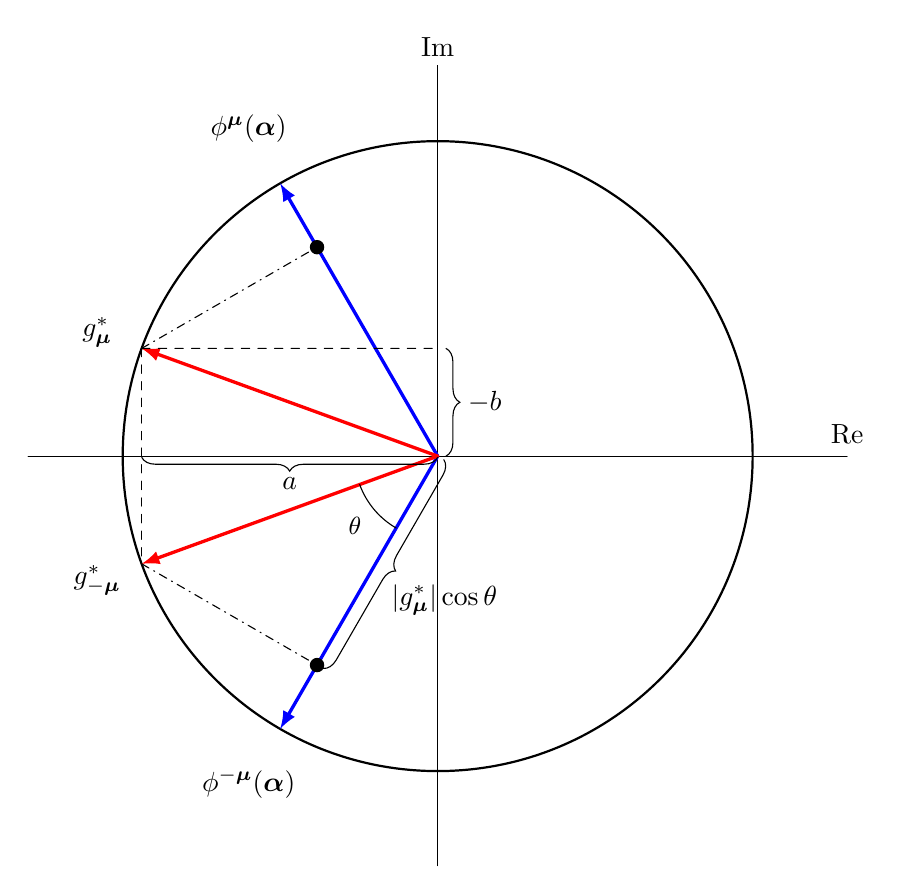
\begin{tikzpicture}[scale=4,cap=round,>=latex]
        % draw the coordinates
        \draw[] (-1.3cm,0cm) -- (1.3cm,0cm) node[right,fill=white] {};
        \draw[] (0cm,-1.3cm) -- (0cm,1.3cm) node[above,fill=white] {};

        % draw the unit circle
        \draw[thick] (0cm,0cm) circle(1cm);

        %coordinates for angle
        \coordinate (O) at (0,0);
        \coordinate (G) at (200:1cm);
        \coordinate (P) at (240:1cm);

        %phi_mu
        \draw[blue, ->, very thick] (0cm,0cm) -- (120:1cm);
        \draw (120:1.2cm) node[fill=white] {$\phi^{\boldsymbol{\mu}}(\boldsymbol{\alpha})$};
    
        %phi_-mu
        \draw[blue, ->, very thick] (0cm,0cm) -- (240:1cm);
        \draw (240:1.2cm) node[fill=white] {$\phi^{-\boldsymbol{\mu}}(\boldsymbol{\alpha})$};

        %g1
        %\draw[red, ->, very thick, dashed] (0cm,0cm) -- (260:1cm);
        %\draw (260:1.2cm) node[fill=white] {$g_\mu$};

        %g_mu*
        \draw[red, ->, very thick] (0cm,0cm) -- (160:1cm);
        \draw (160:1.15cm) node[fill=white] {$g_{\boldsymbol{\mu}}^*$};

        %g_-mu*
        \draw[red, ->, very thick] (0cm,0cm) -- (200:1cm);
        \draw (200:1.15cm) node[fill=white] {$g_{-\boldsymbol{\mu}}^*$};

        %a1
        %\draw[dashed] (100:1cm) -- (260:1cm);
        \draw[dashed] (160:1cm) -- (200:1cm);
        \draw [decorate,decoration={brace,amplitude=5pt,raise=0.1ex}]
        (0,0) -- (-0.939692,0) node[midway,yshift=-1em]{$a$};

        %b1
        %\draw[dashed] (260:1cm) -- (270: .9848cm);
        %\draw [decorate,decoration={brace,amplitude=5pt,raise=0.7ex}]
        %(0,0) -- (0,-.9848) node[midway,xshift=.4cm]{$b$};

        %b1 tilde
        \draw[dashed] (160:1cm) -- (90: .3420cm);
        \draw [decorate,decoration={brace,amplitude=5pt, mirror,raise=0.7ex}]
        (0,0) -- (0,.3420) node[midway,xshift=.6cm]{$-b$};

        %projection
        \draw[dashdotted] (160:1cm) -- (120:.7660cm);
        \filldraw[black] (120:.7660cm) circle(0.6pt);
        %\draw [decorate,decoration={brace,amplitude=5pt, mirror,raise=1ex}]
        %(0,0) -- (120:.7660) node[midway,xshift=1.3cm, yshift=0.6cm]{$|g_{\boldsymbol{\mu}}^*| \cos \theta$};

        \draw[dashdotted] (200:1cm) -- (240:.7660cm);
        \filldraw[black] (240:.7660cm) circle(0.6pt);
        \draw pic[-,"\small $\theta$",draw=black,angle radius=30,angle eccentricity=1.3] {angle=G--O--P};
        \draw [decorate,decoration={brace,amplitude=5pt,raise=0.6ex}]
        (0,0) -- (240:.7660) node[midway,xshift=.85cm, yshift=-.5cm]{$|g_{\boldsymbol{\mu}}^*| \cos \theta$};


        % draw the horizontal and vertical coordinates
        \draw (1.3cm,0cm)  node[above=1pt] {$\Re$}
            (0cm,1.3cm)  node[fill=white] {$\Im$};
    \end{tikzpicture}
    \caption{Contribution of $\phi^{\boldsymbol{\mu}}(\boldsymbol{\alpha})$ to $S(\boldsymbol{\alpha})$ drawn as an inner product.}
    \label{fig:S_a}
\end{figure}

\subsubsection{Parameter inference}

For a complete model, there exists a bijective relation between $p(\boldsymbol{\alpha})$ and the model parameters, which allows us to construct an expression for the model parameters in terms of $p(\boldsymbol{\alpha})$.
Starting from Equation \ref{eq:p_alpha_s_alpha} we can write

\begin{align*}
    \log p(\boldsymbol{\alpha}) &= S(\boldsymbol{\alpha}),\\
    &= \sum_{\boldsymbol{\nu} \in {(\mathbb{Z}/q\mathbb{Z})}^n} g_{\boldsymbol{\nu}} \phi^{\boldsymbol{\nu}}(\boldsymbol{\alpha}),
\end{align*}

\noindent
Multiplying both sides by $\left[\phi^{\boldsymbol{\mu}}(\boldsymbol{\alpha})\right]^*$ and summing over all possible states $\boldsymbol{\alpha}$ gives 

\begin{align*}
    \sum_{\boldsymbol{\alpha} \in {(\mathbb{Z}/q\mathbb{Z})}^n} \left[\phi^{\boldsymbol{\mu}}(\boldsymbol{\alpha})\right]^* \log p(\boldsymbol{\alpha}) &= \sum_{\boldsymbol{\alpha} \in {(\mathbb{Z}/q\mathbb{Z})}^n} \sum_{\boldsymbol{\nu} \in {(\mathbb{Z}/q\mathbb{Z})}^n} g_{\boldsymbol{\nu}} \phi^{\boldsymbol{\nu}}(\boldsymbol{\alpha}) \left[\phi^{\boldsymbol{\mu}}(\boldsymbol{\alpha})\right]^*\\
    &= \sum_{\boldsymbol{\alpha} \in {(\mathbb{Z}/q\mathbb{Z})}^n} g_{\boldsymbol{\mu}} + \sum_{\substack{\boldsymbol{\nu} \in {(\mathbb{Z}/q\mathbb{Z})}^n \\ \boldsymbol{\nu} \neq \boldsymbol{\mu}}} g_{\boldsymbol{\nu}} \sum_{\boldsymbol{\alpha} \in {(\mathbb{Z}/q\mathbb{Z})}^n} \phi^{\boldsymbol{\nu} - \boldsymbol{\mu}}(\boldsymbol{\alpha})
\end{align*}

\noindent
Given that the $\sum_{\boldsymbol{\alpha} \in {(\mathbb{Z}/q\mathbb{Z})}^n} \phi^{\boldsymbol{\mu}} = 0 \quad \forall \boldsymbol{\mu} \neq \mathbf{0}$, we obtain that

\begin{align*}
    g_{\boldsymbol{\mu}} = \frac{1}{q^n}  \sum_{\boldsymbol{\alpha} \in {(\mathbb{Z}/q\mathbb{Z})}^n} \left[\phi^{\boldsymbol{\mu}}(\boldsymbol{\alpha})\right]^* \log p(\boldsymbol{\alpha})
\end{align*}
\clearpage

\subsubsection{Minimally Complex models}

As $\Omega_n \setminus \{ \phi^0 \}$ contains $2^n-1$ operators, we can construct $2^{2^n-1}$ different spin models.
For most systems, searching for the best model among all possible models is unfeasible.
Therefore, the search is usually limited to of a subset of models.
One subset that is commonly used is the set of pairwise models where only interactions upto second-order are considered.
Another subset is the set of minimally complex models (MCMs).
An MCM is defined as the union of independent complete components (ICCs).
A given component, $\mathcal{M}_a$, is called complete if

\begin{equation}
    \mu \oplus \nu \in \mathcal{M}_a \: \forall \: \mu, \nu \in \mathcal{M}_a.
\end{equation}

\noindent
A component is called independent from other components if every operator in the component can only be constructed using operators from the same component.

\subsection{Bayesian model selection}

In Bayesian model selection the model that best fits the data corresponds to the model with the largest posterior probability, $P(\mathcal{M} | \mathbf{\hat{s}})$, which is the probability of the model given the dataset $\mathbf{\hat{s}} = (\mathbf{s}^{(1)} \dots \mathbf{s}^{(N)})$ containing N observed configurations.
Using Bayes' theorem, the posterior probability can be expressed in terms of the evidence, $P(\mathbf{\hat{s}}|\mathcal{M})$, which is the likelihood of the model given the observed dataset.

\begin{equation}
    P(\mathcal{M} | \mathbf{\hat{s}}) = \frac{P(\mathbf{\hat{s}}|\mathcal{M}) \: P(\mathcal{M}) }{\sum_{\mathcal{M}^\prime}P(\mathbf{\hat{s}}|\mathcal{M}^\prime) \: P(\mathcal{M}^\prime)}
\end{equation}

\noindent
The sum in the denominator runs of all the different models that we consider and $P(\mathcal{M})$ is the prior probability of the model.
Without a preference for any model before the observed data, we choose a uniform prior distribution.
As a consequence, the model with the largest evidence will be the model with the largest posterior probability.
Because the likelihood of the model depends on the chosen model parameters, $g_\mu$, we can write is as

\begin{align}
    P(\mathbf{\hat{s}}|\mathcal{M}) &= \int d\mathbf{g} P(\mathbf{\hat{s}} | \mathbf{g}, \mathcal{M}) P_0(\mathbf{g}|\mathcal{M}), \\
    &= \int d\mathbf{g} \prod_{i=1}^N P(\mathbf{s}^{(i)} | \mathbf{g}, \mathcal{M}) P_0(\mathbf{g}|\mathcal{M}). \notag
\end{align}

\noindent
The probability of a single observations $\mathbf{s}^{(i)}$ for a given model and model parameters is the probability defined in Equation \ref{eq:prob_distr}, which allows us to rewrite the evidence as

\begin{align*}
    P(\mathbf{\hat{s}}|\mathcal{M}) &= \int d\mathbf{g} \prod_{i=1}^N \frac{1}{Z_\mathbf{g}(\mathcal{M})} \text{exp}\left(\sum_{\mu \in \mathcal{M}} g_\mu \phi^\mu(\mathbf{s}^{(i)}) \right) P_0(\mathbf{g}|\mathcal{M}), \\
    &= \int d\mathbf{g} \prod_{i=1}^N \text{exp}\left(\sum_{\mu \in \mathcal{M}} \left[ g_\mu \phi^\mu(\mathbf{s}^{(i)}) - \log {Z_\mathbf{g}(\mathcal{M})} \right] \right) P_0(\mathbf{g}|\mathcal{M}), \\
    &= \int d\mathbf{g} \: \text{exp}\left(\sum_{i=1}^N \sum_{\mu \in \mathcal{M}} \left[ g_\mu \phi^\mu(\mathbf{s}^{(i)}) - \log {Z_\mathbf{g}(\mathcal{M})} \right] \right) P_0(\mathbf{g}|\mathcal{M}), \\
    &= \int d\mathbf{g} \: \text{exp}\left(\sum_{\mu \in \mathcal{M}} g_\mu \sum_{i=1}^N \left[ \phi^\mu(\mathbf{s}^{(i)}) - \log {Z_\mathbf{g}(\mathcal{M})} \right] \right) P_0(\mathbf{g}|\mathcal{M}), \\
    &= \int d\mathbf{g} \: \text{exp}\left(\sum_{\mu \in \mathcal{M}} g_\mu N \left[ \phi^\mu(\mathbf{\hat{s}}) - \log {Z_\mathbf{g}(\mathcal{M})} \right] \right) P_0(\mathbf{g}|\mathcal{M}),
\end{align*}

\noindent
where $\phi^\mu(\mathbf{\hat{s}})$ is the empirical average of the operator $\phi^\mu$.

\begin{equation}
    \phi^\mu(\mathbf{\hat{s}}) = \frac{1}{N} \sum_{i=1}^N \phi^\mu(\mathbf{s}^{(i)})
\end{equation}

\noindent
Defining $\boldsymbol{\phi}(\mathbf{\hat{s}})$ as a vector of length $|\mathcal{M}|$ with the entries of $\phi^\mu(\mathbf{\hat{s}})$ for every operator $\mu$, gives the following expression for the evidence of the model

\begin{equation} \label{eq:evidence}
    P(\mathbf{\hat{s}}|\mathcal{M}) = \int d\mathbf{g} \: \text{exp}\left( N  \left[ \mathbf{g} \cdot \boldsymbol{\phi}(\mathbf{\hat{s}}) - \log {Z_\mathbf{g}(\mathcal{M})} \right] \right) P_0(\mathbf{g}|\mathcal{M}).
\end{equation}

\noindent
In this expression we can recognize the log-likelihood of the model parameters given the observed dataset,

\begin{equation} \label{eq:log_likelihood}
    \log P(\mathbf{\hat{s}} | \mathbf{g}, \mathcal{M}) = N  \left[ \mathbf{g} \cdot \boldsymbol{\phi}(\mathbf{\hat{s}}) - \log {Z_\mathbf{g}(\mathcal{M})} \right].
\end{equation}

\noindent
In Appendix \ref{sec:max_log_likelihood} it is shown that for the model parameters that maximize the log-likelihood the expected value for every spin operator considered in the model is equal to the empirical average of that spin operator, which are exactly the used constraints in the construction of the probability distribution that maximizes the entropy.

If the number of observations is large, we can approximate the integral in Equation \ref{eq:evidence} using Laplace's method because the integral will be sharply peaked around the maximum with respect to the model parameters.
The derivation is given in Appendix \ref{sec:laplace} and allows us to write the log-evidence as

\begin{equation}
    \log P(\mathbf{\hat{s}}|\mathcal{M}) \approx \log P(\mathbf{\hat{s}} | \mathbf{g}^\star, \mathcal{M}) -  \frac{|\mathcal{M}|}{2} \log \frac{N}{2 \pi} - \log \left[ \frac{\sqrt{\text{det } \mathbb{J}(\mathbf{g}^\star)}}{P_0(\mathbf{g}^\star|\mathcal{M})} \right]
\end{equation}



% Appendix
\appendix

\newpage

\section{Derivations}

\subsection{Maximum entropy models}\label{sec:max_entropy}

The Shannon entropy is defined as 

\begin{equation}
    S = - \sum_{\mathbf{s}} p(\mathbf{s}) \: \log(p(\mathbf{s})).
\end{equation}

\noindent
The first constraint is the normalization of the distribution,

\begin{equation*}
    \sum_{\mathbf{s}} p(\mathbf{s}) = 1
\end{equation*}

\noindent
Next, we have a set of constraints to make sure that the expected value for every spin operator $\phi^\mu$ in the model corresponds to the observed average value of that spin operator,

\begin{equation*}
    \sum_{\mathbf{s}} \phi^\mu p(\mathbf{s}) = \expval{\phi^\mu}_{data}. \label{eq:constraints}
\end{equation*}

\noindent
To find a probability distribution that maximizes the entropy while satisfying the constraints we can construct the following Lagrangian function and set the derivative with respect to $p(\mathbf{s})$ equal to zero.

\begin{equation}
    \mathcal{L}[p(\mathbf{s})] = S[p(\mathbf{s})] + \lambda_0 \left( \sum_{\mathbf{s}} p(\mathbf{s}) - 1 \right) + \sum_{\mu \in \mathcal{M}} \alpha_\mu \left( \sum_{\mathbf{s}} \phi^\mu \: p(\mathbf{s}) - \expval{\phi^\mu}_{data} \right)\\
\end{equation}

\noindent
The derivative of $\mathcal{L}[p(\mathbf{s})]$ with respect to $p(\mathbf{s})$ is

\begin{equation*}
    \frac{\partial \mathcal{L}[\mathbf{p}]}{\partial p_\mathbf{s}} = \frac{\partial S[\mathbf{p}]}{\partial p_\mathbf{s}} + \lambda_0 \left( \frac{\partial \left( \sum_{\mathbf{s}} p(\mathbf{s}) - 1 \right)}{\partial p_\mathbf{s}}\right) + \sum_{\mu \in \mathcal{M}} \alpha_\mu \left( \frac{\partial \left( \sum_{\mathbf{s}} \phi^\mu \: p(\mathbf{s}) - \expval{\phi^\mu}_{data} \right)}{\partial p_\mathbf{s}} \right) \\
\end{equation*}

\noindent
For the first term on the right-hand side we find

\begin{align*}
    \frac{\partial S[\mathbf{p}]}{\partial p_\mathbf{s}} &= - \frac{\partial \sum_{\mathbf{s}} p(\mathbf{s}) \: \log(p(\mathbf{s}))}{\partial p_\mathbf{s}}\\
    &= - \frac{\partial \: p_{\mathbf{s}} \: \log(p_{\mathbf{s}})}{\partial p_\mathbf{s}} \\
    &= - \log(p_{\mathbf{s}}) \frac{\partial p_\mathbf{s}}{\partial p_\mathbf{s}} - p_\mathbf{s} \frac{\partial \log(p_\mathbf{s})}{\partial p_\mathbf{s}} \\
    &= - \log(p_{\mathbf{s}}) - 1 \notag
\end{align*}

\noindent
For the second term on the right-hand side we find

\begin{align*}
    \lambda_0 \left( \frac{\partial \left( \sum_{\mathbf{s}} p(\mathbf{s}) - 1 \right)}{\partial p_\mathbf{s}}\right) &= \lambda_0 \left( \frac{\partial \sum_{\mathbf{s}} p(\mathbf{s})}{\partial p_\mathbf{s}} -  \frac{\partial \: 1}{{\partial p_\mathbf{s}}}\right) \\
    &= \lambda_0 \left(\frac{\partial p_\mathbf{s}}{\partial p_\mathbf{s}} - 0 \right) \\
    &= \lambda_0 \notag
\end{align*}

\noindent
For the last term on the right-hand side we find

\begin{align*}
    \sum_{\mu \in \mathcal{M}} \alpha_\mu \left( \frac{\partial \left( \sum_{\mathbf{s}} \phi^\mu \: p(\mathbf{s}) - \expval{\phi^\mu}_{data} \right)}{\partial p_\mathbf{s}} \right) &= \sum_{\mu \in \mathcal{M}} \alpha_\mu \left( \frac{\partial \sum_{\mathbf{s}} \phi^\mu(\mathbf{s}) p(\mathbf{s})}{\partial p_\mathbf{s}} - \frac{\partial \expval{\phi^\mu}_{data}}{\partial p_\mathbf{s}} \right)\\
    &= \sum_{\mu \in \mathcal{M}} \alpha_\mu \left( \frac{\partial \phi^\mu(\mathbf{s}) p_{\mathbf{s}}}{\partial p_\mathbf{s}} - 0\right) \\
    &= \sum_{\mu \in \mathcal{M}} \alpha_\mu \phi^\mu(\mathbf{s})
\end{align*}

\noindent
Then, the final expression for the derivative of $\mathcal{L}[p(\mathbf{s})]$ with respect to $p(\mathbf{s})$ is

\begin{equation}
    \frac{\partial \mathcal{L}[\mathbf{p}]}{\partial p_\mathbf{s}} = - \log(p_{\mathbf{s}}) - 1 + \lambda_0 + \sum_{\mu \in \mathcal{M}} \alpha_\mu \phi^\mu(\mathbf{s}).
\end{equation}

\noindent
Setting the derivative of $\mathcal{L}[p(\mathbf{s})]$ with respect to $p(\mathbf{s})$ equal to zero gives the desired form of the probability distribution.

\begin{align*}
    0 &= \frac{\partial \mathcal{L}[\mathbf{p}]}{\partial p_\mathbf{s}}\\
    0 &= - \log(p_{\mathbf{s}}) - 1 + \lambda_0 + \sum_{\mu \in \mathcal{M}} \alpha_\mu \phi^\mu(\mathbf{s}) \\
    \log(p_{\mathbf{s}}) &= - 1 + \lambda_0 + \sum_{\mu \in \mathcal{M}} \alpha_\mu \phi^\mu(\mathbf{s})\\
    p_{\mathbf{s}} &= e^{\lambda_0 - 1 + \sum_{\mu \in \mathcal{M}} \alpha_\mu \phi^\mu(\mathbf{s})}\\
    &= e^{\lambda_0 - 1} e^{ \sum_{\mu \in \mathcal{M}} \alpha_\mu \phi^\mu(\mathbf{s})}
\end{align*}

\noindent
This expression has the same form as the expression in Equation \ref{eq:prob_distr}. The lagrange multipliers $\alpha_\mu$ have a one-to-one correspondence to interaction strength, $g_\mu$.
Then, the expression for the partition function becomes

\begin{equation*}
    Z = e^{1 - \lambda_0}.
\end{equation*}

\noindent
Knowing that the probability distribution is normalized this expression can be rewritten,

\begin{align*}
  &\sum_{\mathbf{s}} p_{\mathbf{s}} = 1, \\
  &\sum_{\mathbf{s}}  e^{\lambda_0 - 1} e^{\sum_{\mu \in \mathcal{M}} g_\mu \phi^\mu(\mathbf{s})} = 1, \\
  &e^{\lambda_0 - 1} = \frac{1}{\sum_{\mathbf{s}} e^{\sum_{\mu \in \mathcal{M}} g_\mu \phi^\mu(\mathbf{s})}},
\end{align*}

\noindent
which yields the final form of the probability distribution

\begin{equation}
  p_{\mathbf{g}}(\mathbf{s}) = \frac{e^{\sum_{\mu \in \mathcal{M}} g_\mu \phi^\mu(\mathbf{s})}}{\sum_{\mathbf{s}} e^{\sum_{\mu \in \mathcal{M}} g_\mu \phi^\mu(\mathbf{s})}}.
\end{equation}

\begin{landscape}
\newgeometry{top=2.5cm, left=2cm,bottom=1cm, right=2cm}
\subsection{Spin operator matrix three-state system with two spins} \label{sec:discrete_spin_op_matrix}

\begin{align*}
    & \hspace{-.2cm} \scriptstyle \mathbf{S}^{(3)} \otimes \mathbf{S}^{(3)} = \\
    & \hspace{-.3cm} \begin{bmatrix}
        \phi^0(\alpha=0) & \phi^1(\alpha=0) & {(\phi^1)}^2(\alpha=0)\\
        \phi^0(\alpha=1) & \phi^1(\alpha=1) & {(\phi^1)}^2(\alpha=1)\\
        \phi^0(\alpha=2) & \phi^1(\alpha=2) & {(\phi^1)}^2(\alpha=2)\\
    \end{bmatrix} \otimes \begin{bmatrix}
        \phi^0(\alpha=0) & \phi^1(\alpha=0) & {(\phi^1)}^2(\alpha=0)\\
        \phi^0(\alpha=1) & \phi^1(\alpha=1) & {(\phi^1)}^2(\alpha=1)\\
        \phi^0(\alpha=2) & \phi^1(\alpha=2) & {(\phi^1)}^2(\alpha=2)\\
    \end{bmatrix}=\\
    & \hspace{-.3cm} \begin{bmatrix}
        \scriptstyle \phi^0(\alpha_2=0) \phi^0(\alpha_1=0) & \hspace{-4pt} \scriptstyle \phi^0(\alpha_2=0) \phi^1(\alpha_1=0) & \hspace{-4pt} \scriptstyle \phi^0(\alpha_2=0) {(\phi^1)}^2(\alpha_1=0) & \hspace{-4pt} \scriptstyle \phi^1(\alpha_2=0) \phi^0(\alpha_1=0) & \hspace{-4pt} \scriptstyle \phi^1(\alpha_2=0) \phi^1(\alpha_1=0) & \hspace{-4pt} \scriptstyle \phi^1(\alpha_2=0) {(\phi^1)}^2(\alpha_1=0) & \hspace{-4pt} \scriptstyle {(\phi^1)}^2(\alpha_2=0) \phi^0(\alpha_1=0) & \hspace{-4pt} \scriptstyle {(\phi^1)}^2(\alpha_2=0) \phi^1(\alpha_1=0) & \hspace{-4pt} \scriptstyle {(\phi^1)}^2(\alpha_2=0) {(\phi^1)}^2(\alpha_1=0) \\ 
        \scriptstyle \phi^0(\alpha_2=0) \phi^0(\alpha_1=1) & \hspace{-4pt} \scriptstyle \phi^0(\alpha_2=0) \phi^1(\alpha_1=1) & \hspace{-4pt} \scriptstyle \phi^0(\alpha_2=0) {(\phi^1)}^2(\alpha_1=1) & \hspace{-4pt} \scriptstyle \phi^1(\alpha_2=0) \phi^0(\alpha_1=1) & \hspace{-4pt} \scriptstyle \phi^1(\alpha_2=0) \phi^1(\alpha_1=1) & \hspace{-4pt} \scriptstyle \phi^1(\alpha_2=0) {(\phi^1)}^2(\alpha_1=1) & \hspace{-4pt} \scriptstyle {(\phi^1)}^2(\alpha_2=0) \phi^0(\alpha_1=1) & \hspace{-4pt} \scriptstyle {(\phi^1)}^2(\alpha_2=0) \phi^1(\alpha_1=1) & \hspace{-4pt} \scriptstyle {(\phi^1)}^2(\alpha_2=0) {(\phi^1)}^2(\alpha_1=1) \\
        \scriptstyle \phi^0(\alpha_2=0) \phi^0(\alpha_1=2) & \hspace{-4pt} \scriptstyle \phi^0(\alpha_2=0) \phi^1(\alpha_1=2) & \hspace{-4pt} \scriptstyle \phi^0(\alpha_2=0) {(\phi^1)}^2(\alpha_1=2) & \hspace{-4pt} \scriptstyle \phi^1(\alpha_2=0) \phi^0(\alpha_1=2) & \hspace{-4pt} \scriptstyle \phi^1(\alpha_2=0) \phi^1(\alpha_1=2) & \hspace{-4pt} \scriptstyle \phi^1(\alpha_2=0) {(\phi^1)}^2(\alpha_1=2) & \hspace{-4pt} \scriptstyle {(\phi^1)}^2(\alpha_2=0) \phi^0(\alpha_1=2) & \hspace{-4pt} \scriptstyle {(\phi^1)}^2(\alpha_2=0) \phi^1(\alpha_1=2) & \hspace{-4pt} \scriptstyle {(\phi^1)}^2(\alpha_2=0) {(\phi^1)}^2(\alpha_1=2) \\ 
        \scriptstyle \phi^0(\alpha_2=1) \phi^0(\alpha_1=0) & \hspace{-4pt} \scriptstyle \phi^0(\alpha_2=1) \phi^1(\alpha_1=0) & \hspace{-4pt} \scriptstyle \phi^0(\alpha_2=1) {(\phi^1)}^2(\alpha_1=0) & \hspace{-4pt} \scriptstyle \phi^1(\alpha_2=1) \phi^0(\alpha_1=0) & \hspace{-4pt} \scriptstyle \phi^1(\alpha_2=1) \phi^1(\alpha_1=0) & \hspace{-4pt} \scriptstyle \phi^1(\alpha_2=1) {(\phi^1)}^2(\alpha_1=0) & \hspace{-4pt} \scriptstyle {(\phi^1)}^2(\alpha_2=1) \phi^0(\alpha_1=0) & \hspace{-4pt} \scriptstyle {(\phi^1)}^2(\alpha_2=1) \phi^1(\alpha_1=0) & \hspace{-4pt} \scriptstyle {(\phi^1)}^2(\alpha_2=1) {(\phi^1)}^2(\alpha_1=0) \\ 
        \scriptstyle \phi^0(\alpha_2=1) \phi^0(\alpha_1=1) & \hspace{-4pt} \scriptstyle \phi^0(\alpha_2=1) \phi^1(\alpha_1=1) & \hspace{-4pt} \scriptstyle \phi^0(\alpha_2=1) {(\phi^1)}^2(\alpha_1=1) & \hspace{-4pt} \scriptstyle \phi^1(\alpha_2=1) \phi^0(\alpha_1=1) & \hspace{-4pt} \scriptstyle \phi^1(\alpha_2=1) \phi^1(\alpha_1=1) & \hspace{-4pt} \scriptstyle \phi^1(\alpha_2=1) {(\phi^1)}^2(\alpha_1=1) & \hspace{-4pt} \scriptstyle {(\phi^1)}^2(\alpha_2=1) \phi^0(\alpha_1=1) & \hspace{-4pt} \scriptstyle {(\phi^1)}^2(\alpha_2=1) \phi^1(\alpha_1=1) & \hspace{-4pt} \scriptstyle {(\phi^1)}^2(\alpha_2=1) {(\phi^1)}^2(\alpha_1=1) \\ 
        \scriptstyle \phi^0(\alpha_2=1) \phi^0(\alpha_1=2) & \hspace{-4pt} \scriptstyle \phi^0(\alpha_2=1) \phi^1(\alpha_1=2) & \hspace{-4pt} \scriptstyle \phi^0(\alpha_2=1) {(\phi^1)}^2(\alpha_1=2) & \hspace{-4pt} \scriptstyle \phi^1(\alpha_2=1) \phi^0(\alpha_1=2) & \hspace{-4pt} \scriptstyle \phi^1(\alpha_2=1) \phi^1(\alpha_1=2) & \hspace{-4pt} \scriptstyle \phi^1(\alpha_2=1) {(\phi^1)}^2(\alpha_1=2) & \hspace{-4pt} \scriptstyle {(\phi^1)}^2(\alpha_2=1) \phi^0(\alpha_1=2) & \hspace{-4pt} \scriptstyle {(\phi^1)}^2(\alpha_2=1) \phi^1(\alpha_1=2) & \hspace{-4pt} \scriptstyle {(\phi^1)}^2(\alpha_2=1) {(\phi^1)}^2(\alpha_1=2) \\
        \scriptstyle \phi^0(\alpha_2=2) \phi^0(\alpha_1=0) & \hspace{-4pt} \scriptstyle \phi^0(\alpha_2=2) \phi^1(\alpha_1=0) & \hspace{-4pt} \scriptstyle \phi^0(\alpha_2=2) {(\phi^1)}^2(\alpha_1=0) & \hspace{-4pt} \scriptstyle \phi^1(\alpha_2=2) \phi^0(\alpha_1=0) & \hspace{-4pt} \scriptstyle \phi^1(\alpha_2=2) \phi^1(\alpha_1=0) & \hspace{-4pt} \scriptstyle \phi^1(\alpha_2=2) {(\phi^1)}^2(\alpha_1=0) & \hspace{-4pt} \scriptstyle {(\phi^1)}^2(\alpha_2=2) \phi^0(\alpha_1=0) & \hspace{-4pt} \scriptstyle {(\phi^1)}^2(\alpha_2=2) \phi^1(\alpha_1=0) & \hspace{-4pt} \scriptstyle {(\phi^1)}^2(\alpha_2=2) {(\phi^1)}^2(\alpha_1=0) \\
        \scriptstyle \phi^0(\alpha_2=2) \phi^0(\alpha_1=1) & \hspace{-4pt} \scriptstyle \phi^0(\alpha_2=2) \phi^1(\alpha_1=1) & \hspace{-4pt} \scriptstyle \phi^0(\alpha_2=2) {(\phi^1)}^2(\alpha_1=1) & \hspace{-4pt} \scriptstyle \phi^1(\alpha_2=2) \phi^0(\alpha_1=1) & \hspace{-4pt} \scriptstyle \phi^1(\alpha_2=2) \phi^1(\alpha_1=1) & \hspace{-4pt} \scriptstyle \phi^1(\alpha_2=2) {(\phi^1)}^2(\alpha_1=1) & \hspace{-4pt} \scriptstyle {(\phi^1)}^2(\alpha_2=2) \phi^0(\alpha_1=1) & \hspace{-4pt} \scriptstyle {(\phi^1)}^2(\alpha_2=2) \phi^1(\alpha_1=1) & \hspace{-4pt} \scriptstyle {(\phi^1)}^2(\alpha_2=2) {(\phi^1)}^2(\alpha_1=1) \\
        \scriptstyle \phi^0(\alpha_2=2) \phi^0(\alpha_1=2) & \hspace{-4pt} \scriptstyle \phi^0(\alpha_2=2) \phi^1(\alpha_1=2) & \hspace{-4pt} \scriptstyle \phi^0(\alpha_2=2) {(\phi^1)}^2(\alpha_1=2) & \hspace{-4pt} \scriptstyle \phi^1(\alpha_2=2) \phi^0(\alpha_1=2) & \hspace{-4pt} \scriptstyle \phi^1(\alpha_2=2) \phi^1(\alpha_1=2) & \hspace{-4pt} \scriptstyle \phi^1(\alpha_2=2) {(\phi^1)}^2(\alpha_1=2) & \hspace{-4pt} \scriptstyle {(\phi^1)}^2(\alpha_2=2) \phi^0(\alpha_1=2) & \hspace{-4pt} \scriptstyle {(\phi^1)}^2(\alpha_2=2) \phi^1(\alpha_1=2) & \hspace{-4pt} \scriptstyle {(\phi^1)}^2(\alpha_2=2) {(\phi^1)}^2(\alpha_1=2)  
    \end{bmatrix}\scriptstyle = \hspace{-.7cm}\\
    & \hspace{-.3cm} \begin{bmatrix}
        1 & 1 & 1 & 1 & 1 & 1 & 1 & 1 & 1 \\
        1 & e^{-\frac{2\pi i}{3}} & e^{-\frac{4\pi i}{3}} & 1 & e^{-\frac{2\pi i}{3}} & e^{-\frac{4\pi i}{3}} & 1 & e^{-\frac{2\pi i}{3}} & e^{-\frac{4\pi i}{3}} \\
        1 & e^{-\frac{4\pi i}{3}} & e^{-\frac{2\pi i}{3}} & 1 & e^{-\frac{4\pi i}{3}} & e^{-\frac{2\pi i}{3}} & 1 & e^{-\frac{4\pi i}{3}} & e^{-\frac{2\pi i}{3}} \\
        1 & 1 & 1 & e^{-\frac{2\pi i}{3}} & e^{-\frac{2\pi i}{3}} & e^{-\frac{2\pi i}{3}} & e^{-\frac{4\pi i}{3}} & e^{-\frac{4\pi i}{3}} & e^{-\frac{4\pi i}{3}} \\
        1 & e^{-\frac{2\pi i}{3}} & e^{-\frac{4\pi i}{3}} & e^{-\frac{2\pi i}{3}} & e^{-\frac{4\pi i}{3}} & 1 & e^{-\frac{4\pi i}{3}} & 1 & e^{-\frac{2\pi i}{3}} \\
        1 & e^{-\frac{4\pi i}{3}} & e^{-\frac{2\pi i}{3}} & e^{-\frac{2\pi i}{3}} & 1 & e^{-\frac{4\pi i}{3}} & e^{-\frac{4\pi i}{3}} & e^{-\frac{2\pi i}{3}} & 1 \\
        1 & 1 & 1 & e^{-\frac{4\pi i}{3}} & e^{-\frac{4\pi i}{3}} & e^{-\frac{4\pi i}{3}} & e^{-\frac{2\pi i}{3}} & e^{-\frac{2\pi i}{3}} & e^{-\frac{2\pi i}{3}} \\
        1 & e^{-\frac{2\pi i}{3}} & e^{-\frac{4\pi i}{3}} & e^{-\frac{4\pi i}{3}} & 1 & e^{-\frac{2\pi i}{3}} & e^{-\frac{2\pi i}{3}} & e^{-\frac{4\pi i}{3}} & 1 \\
        1 & e^{-\frac{4\pi i}{3}} & e^{-\frac{2\pi i}{3}} & e^{-\frac{4\pi i}{3}} & e^{-\frac{2\pi i}{3}} & 1 & e^{-\frac{2\pi i}{3}} & 1 & e^{-\frac{4\pi i}{3}} \\
    \end{bmatrix}\\
\end{align*}
\restoregeometry
\end{landscape}

\subsection{Expected values at maximum log-likelihood} \label{sec:max_log_likelihood}

Setting the derivative of the log-likelihood in Equation \ref{eq:log_likelihood} with respect to the model parameters $g_\mu$ equal to zero gives,

\begin{align*}
    0 &= \frac{\partial \log P(\mathbf{\hat{s}} | \mathbf{g}, \mathcal{M})}{\partial g_\mu}, \\
    &= N \frac{\partial  \mathbf{g} \cdot \mathbf{\phi}(\mathbf{\hat{s}}) - \log {Z_\mathbf{g}(\mathcal{M})}}{\partial g_\mu}, \\
    &= N \left[ \phi^\mu(\mathbf{\hat{s}}) - \frac{1}{Z_\mathbf{g}(\mathcal{M})} \frac{\partial {Z_\mathbf{g}(\mathcal{M})}}{\partial g_\mu} \right], \\
    &= N \left[ \phi^\mu(\mathbf{\hat{s}}) - \frac{1}{Z_\mathbf{g}(\mathcal{M})} \frac{\partial \sum_{\mathbf{s} \in \mathbf{\hat{s}}} e^{\left(\sum_{\mu \in \mathcal{M}} g_\mu \phi^\mu(\mathbf{s}) \right)}}{\partial g_\mu} \right], \\
    &= N \left[ \phi^\mu(\mathbf{\hat{s}}) - \frac{1}{Z_\mathbf{g}(\mathcal{M})} \sum_{\mathbf{s} \in \mathbf{\hat{s}}} \phi^\mu(\mathbf{s}) e^{\left(\sum_{\mu \in \mathcal{M}} g_\mu \phi^\mu(\mathbf{s}) \right)} \right], \\
    &= N \left[ \phi^\mu(\mathbf{\hat{s}}) - \sum_{\mathbf{s} \in \mathbf{\hat{s}}} \phi^\mu(\mathbf{s}) P(\mathbf{s} | \mathbf{g}, \mathcal{M})\right],
\end{align*}

\noindent
which shows that at the maximum of the log-likelihood

\begin{equation}
  \phi^\mu(\mathbf{\hat{s}}) = \sum_{\mathbf{s} \in \mathbf{\hat{s}}} \phi^\mu(\mathbf{s}) P(\mathbf{s} | \mathbf{g}, \mathcal{M}).
\end{equation}

\subsection{Expression for evidence using Laplace's method} \label{sec:laplace}

Because the value of the integral in Equation \ref{eq:evidence} is dominated by a single contribution at the maximum, we can replace the term in the exponential by its second-order Taylor expansion around the model parameters, $\mathbf{g}^\star$, that maximize the evidence.

\begin{align*}
  N  \left[ \mathbf{g} \cdot \mathbf{\phi}(\mathbf{\hat{s}}) - \log {Z_\mathbf{g}(\mathcal{M})} \right] \approx& \: N  \left[ \mathbf{g}^\star \cdot \mathbf{\phi}(\mathbf{\hat{s}}) - \log {Z_\mathbf{g^\star}(\mathcal{M})} \right] + (\mathbf{g} - \mathbf{g}^\star)^\intercal \nabla \bigl[ N  \left[ \mathbf{g} \cdot \mathbf{\phi}(\mathbf{\hat{s}}) - \log {Z_\mathbf{g}(\mathcal{M})} \right] \bigr](\mathbf{g}^\star) \\
&+ \frac{1}{2}  (\mathbf{g} - \mathbf{g}^\star)^\intercal \nabla^2 \bigl[ N  \left[ \mathbf{g} \cdot \mathbf{\phi}(\mathbf{\hat{s}}) - \log {Z_\mathbf{g}(\mathcal{M})} \right] \bigr] (\mathbf{g}^\star) (\mathbf{g} - \mathbf{g}^\star) \\
=& \log P(\mathbf{\hat{s}} | \mathbf{g}^\star, \mathcal{M}) - \frac{1}{2}  (\mathbf{g} - \mathbf{g}^\star)^\intercal \nabla^2 \bigl[ N \log {Z_\mathbf{g}(\mathcal{M})} \bigr] (\mathbf{g}^\star) (\mathbf{g} - \mathbf{g}^\star)
%=& \log P(\mathbf{\hat{s}} | \mathbf{g}^\star, \mathcal{M}) - \frac{N}{2} (\mathbf{g} - \mathbf{g}^\star)^\intercal \mathbb{J}(\mathbf{g}^\star)(\mathbf{g} - \mathbf{g}^\star)
\end{align*}

%\begin{equation*}
%  P_0(\mathbf{g}|\mathcal{M}) \approx \: P_0(\mathbf{g}^\star|\mathcal{M}) +  (\mathbf{g} - \mathbf{g}^\star)^\intercal \nabla \bigl[ P_0(\mathbf{g}|\mathcal{M})\bigr](\mathbf{g}^\star) + \frac{1}{2} (\mathbf{g} - \mathbf{g}^\star)^\intercal \nabla^2 \bigl[ P_0(\mathbf{g}|\mathcal{M}) \bigr] (\mathbf{g}^\star) (\mathbf{g} - \mathbf{g}^\star)
%\end{equation*}

\noindent
Plugging this expansion into the expression for the evidence and using the definition of the Fisher information matrix, which has as entries

\begin{equation}
    \mathbb{J}_{\mu\nu}(\mathbf{g}) = \frac{\partial^2 \log {Z_\mathbf{g}(\mathcal{M})}}{\partial g_\mu \partial g_\nu},
\end{equation}

\noindent
gives the following expression for the evidence.

\begin{align*}
    P(\mathbf{\hat{s}}|\mathcal{M}) \approx& \int d\mathbf{g} \: e^{\log P(\mathbf{\hat{s}} | \mathbf{g}^\star, \mathcal{M}) - \frac{N}{2}  (\mathbf{g} - \mathbf{g}^\star)^\intercal \mathbb{J} (\mathbf{g}^\star) (\mathbf{g} - \mathbf{g}^\star)} P_0(\mathbf{g}|\mathcal{M}) \\
   =& \int d\mathbf{g} \: P(\mathbf{\hat{s}} | \mathbf{g}^\star, \mathcal{M})  e^{-\frac{N}{2}  (\mathbf{g} - \mathbf{g}^\star)^\intercal \mathbb{J} (\mathbf{g}^\star) (\mathbf{g} - \mathbf{g}^\star)} P_0(\mathbf{g}|\mathcal{M}) \\
   =& P(\mathbf{\hat{s}} | \mathbf{g}^\star, \mathcal{M}) P_0(\mathbf{g}^\star|\mathcal{M}) \int d\mathbf{g} \: e^{-\frac{N}{2}  (\mathbf{g} - \mathbf{g}^\star)^\intercal \mathbb{J} (\mathbf{g}^\star) (\mathbf{g} - \mathbf{g}^\star)} \\
\end{align*}

%\begin{align*}
%    P(\mathbf{\hat{s}}|\mathcal{M}) \approx& \int d\mathbf{g} \: e^{\log P(\mathbf{\hat{s}} | \mathbf{g}^\star, \mathcal{M}) - \frac{N}{2}  (\mathbf{g} - \mathbf{g}^\star)^\intercal \mathbb{J} (\mathbf{g}^\star) (\mathbf{g} - \mathbf{g}^\star)} \\
%    & \left( P_0(\mathbf{g}^\star|\mathcal{M}) +  (\mathbf{g} - \mathbf{g}^\star)^\intercal \nabla \bigl[ P_0(\mathbf{g}|\mathcal{M})\bigr](\mathbf{g}^\star) + \frac{1}{2} (\mathbf{g} - \mathbf{g}^\star)^\intercal \nabla^2 \bigl[ P_0(\mathbf{g}|\mathcal{M}) \bigr] (\mathbf{g}^\star) (\mathbf{g} - \mathbf{g}^\star) \right) \\
%   =& \int d\mathbf{g} \: P(\mathbf{\hat{s}} | \mathbf{g}^\star, \mathcal{M})  e^{-\frac{N}{2}  (\mathbf{g} - \mathbf{g}^\star)^\intercal \mathbb{J} (\mathbf{g}^\star) (\mathbf{g} - \mathbf{g}^\star)} \\
%   &\left( P_0(\mathbf{g}^\star|\mathcal{M}) +  (\mathbf{g} - \mathbf{g}^\star)^\intercal \nabla \bigl[ P_0(\mathbf{g}|\mathcal{M})\bigr](\mathbf{g}^\star) + \frac{1}{2} (\mathbf{g} - \mathbf{g}^\star)^\intercal \nabla^2 \bigl[ P_0(\mathbf{g}|\mathcal{M}) \bigr] (\mathbf{g}^\star) (\mathbf{g} - \mathbf{g}^\star) \right) \\
%   =& P(\mathbf{\hat{s}} | \mathbf{g}^\star, \mathcal{M}) P_0(\mathbf{g}^\star|\mathcal{M}) \int d\mathbf{g} \: e^{-\frac{N}{2}  (\mathbf{g} - \mathbf{g}^\star)^\intercal \mathbb{J} (\mathbf{g}^\star) (\mathbf{g} - \mathbf{g}^\star)} \\
%   &\left(1 + \frac{1}{P_0(\mathbf{g}^\star|\mathcal{M})} (\mathbf{g} - \mathbf{g}^\star)^\intercal \nabla \bigl[ P_0(\mathbf{g}|\mathcal{M})\bigr](\mathbf{g}^\star) + \frac{1}{2 P_0(\mathbf{g}^\star|\mathcal{M})} (\mathbf{g} - \mathbf{g}^\star)^\intercal \nabla^2 \bigl[ P_0(\mathbf{g}|\mathcal{M}) \bigr] (\mathbf{g}^\star) (\mathbf{g} - \mathbf{g}^\star) \right)
%\end{align*}

\noindent
The integral is a multidimensional Gaussian integral. Because the Fisher information matrix is symmetric, we can decompose it as,

\begin{equation*}
    \mathbb{J} = Q \Lambda Q^\intercal,
\end{equation*}

\noindent
where Q is an orthonormal matrix that has the linearly independent eigenvectors of $\mathbb{J}$ as columns. Defining a new variable $\mathbf{x} \equiv Q^\intercal (\mathbf{g} - \mathbf{g}^\star)$, allows us to write the integral as a product of 1D Gaussian integrals.

\begin{align*}
    \int d\mathbf{g} \: e^{-\frac{N}{2}  (\mathbf{g} - \mathbf{g}^\star)^\intercal \mathbb{J} (\mathbf{g}^\star) (\mathbf{g} - \mathbf{g}^\star)} &= \int d\mathbf{g} \: e^{-\frac{N}{2}  (\mathbf{g} - \mathbf{g}^\star)^\intercal Q \Lambda Q^\intercal (\mathbf{g} - \mathbf{g}^\star)}\\
    &= \int d\mathbf{x} \: e^{-\frac{N}{2}  \mathbf{x}^\intercal \Lambda \mathbf{x}} \\
    &= \prod_{\mu = 1}^{|\mathcal{M}|} \int dx_\mu e^{-\frac{N}{2} \lambda_\mu x_\mu^2} \\
    &= \prod_{\mu = 1}^{|\mathcal{M}|} \sqrt{\frac{2 \pi}{N \lambda_\mu}} \\
    &= \left(\frac{2 \pi}{N}\right)^\frac{|\mathcal{M}|}{2} \frac{1}{\sqrt{\text{det } \mathbb{J}(\mathbf{g}^\star)}}
\end{align*}

\noindent
Substituting this into the expression for the log-evidence gives

\begin{align*}
    \log P(\mathbf{\hat{s}}|\mathcal{M}) &\approx \log \left[ P(\mathbf{\hat{s}} | \mathbf{g}^\star, \mathcal{M}) P_0(\mathbf{g}^\star|\mathcal{M}) \left(\frac{2 \pi}{N}\right)^\frac{|\mathcal{M}|}{2}  \frac{1}{\sqrt{\text{det } \mathbb{J}(\mathbf{g}^\star)}} \right]\\
    &= \log P(\mathbf{\hat{s}} | \mathbf{g}^\star, \mathcal{M}) -  \frac{|\mathcal{M}|}{2} \log \frac{N}{2 \pi} - \log \left[ \frac{\sqrt{\text{det } \mathbb{J}(\mathbf{g}^\star)}}{P_0(\mathbf{g}^\star|\mathcal{M})} \right]
\end{align*}
\clearpage
\section{Examples of spin models}

\subsection{2-state,2-spin system}\label{sec:2spin_2states}

Consider a two-spin system and a corresponding complete model. Then, there are 4 different configurations that can be observed and, including $\phi^0$, there are 4 spin operators.
The probability for the 4 different configurations can be written as

\begin{align*}
    p(s_1=1, s_2=1) &= \frac{1}{Z(\mathbf{g})} e^{g_0 \phi^0(s_1=1, s_2=1) + g_1 \phi^1(s_1=1, s_2=1) + g_2 \phi^2(s_1=1, s_2=1) + g_3 \phi^3(s_1=1, s_2=1)},\\
    p(s_1=-1, s_2=1) &= \frac{1}{Z(\mathbf{g})} e^{g_0 \phi^0(s_1=-1, s_2=1) + g_1 \phi^1(s_1=-1, s_2=1) + g_2 \phi^2(s_1=-1, s_2=1) + g_3 \phi^3(s_1=-1, s_2=1)},\\
    p(s_1=1, s_2=-1) &= \frac{1}{Z(\mathbf{g})} e^{g_0 \phi^0(s_1=1, s_2=-1) + g_1 \phi^1(s_1=1, s_2=-1) + g_2 \phi^2(s_1=1, s_2=-1) + g_3 \phi^3(s_1=1, s_2=-1)},\\
    p(s_1=-1, s_2=-1) &= \frac{1}{Z(\mathbf{g})} e^{g_0 \phi^0(s_1=-1, s_2=-1) + g_1 \phi^1(s_1=-1, s_2=-1) + g_2 \phi^2(s_1=-1, s_2=-1) + g_3 \phi^3(s_1=-1, s_2=-1)},\\
\end{align*}

\noindent
which can be rewritten as

\begin{align*}
    p(s_1=1, s_2=1) &= \frac{1}{Z(\mathbf{g})} e^{g_0 + g_1 + g_2 + g_3},\\
    p(s_1=-1, s_2=1) &= \frac{1}{Z(\mathbf{g})} e^{g_0 - g_1 + g_2 - g_3},\\
    p(s_1=1, s_2=-1) &= \frac{1}{Z(\mathbf{g})} e^{g_0 + g_1 - g_2 - g_3},\\
    p(s_1=-1, s_2=-1) &= \frac{1}{Z(\mathbf{g})} e^{g_0 - g_1 - g_2 + g_3}.
\end{align*}

\noindent
In case of a complete model, we can define a spin operator matrix,

\begin{equation}
    \mathbf{S}^{(2)} = \begin{bmatrix}
        \phi^0(s=1) & \phi^1(s=1)\\
        \phi^0(s=-1) & \phi^1(s=-1)
    \end{bmatrix} = \begin{bmatrix}
        1 & 1\\
        1 & -1
    \end{bmatrix},
\end{equation}

\noindent
such that the probability of a configuration can be written as an element of the matrix vector product,

\begin{equation}\label{eq:relation_p_g}
    \mathbf{p} = \exp\left(\bigotimes_{i = 1}^{n} \mathbf{S}^{(2)} \cdot \mathbf{g}\right).
\end{equation}

\noindent
In a two-spin system, the matrix $\bigotimes_{i = 1}^{n} \mathbf{S}^{(2)}$ is equal to

\begin{align*}
    \scriptstyle
    \mathbf{S}^{(2)} \otimes \mathbf{S}^{(2)} &= \begin{bmatrix}
        \phi^0(s_2=1) & \phi^1(s_2=1)\\
        \phi^0(s_2=-1) & \phi^1(s_2=-1)
    \end{bmatrix} \otimes \begin{bmatrix}
        \phi^0(s_1=1) & \phi^1(s_1=1)\\
        \phi^0(s_1=-1) & \phi^1(s_1=-1)
    \end{bmatrix}\\
    &= \begin{bmatrix}
        \scriptstyle \phi^0(s_2=1) \phi^0(s_1=1) & \scriptstyle \phi^0(s_2=1) \phi^1(s_1=1) & \scriptstyle \phi^1(s_2=1) \phi^0(s_1=1) & \scriptstyle \phi^1(s_2=1) \phi^1(s_1=1)\\
        \scriptstyle \phi^0(s_2=1) \phi^0(s_1=-1) & \scriptstyle \phi^0(s_2=1) \phi^1(s_1=-1) & \scriptstyle \phi^1(s_2=1) \phi^0(s_1=-1) & \scriptstyle \phi^1(s_2=1) \phi^1(s_1=-1)\\
        \scriptstyle \phi^0(s_2=-1) \phi^0(s_1=1) & \scriptstyle \phi^0(s_2=-1) \phi^1(s_1=1) & \scriptstyle \phi^1(s_2=-1) \phi^0(s_1=1) & \scriptstyle \phi^1(s_2=-1) \phi^1(s_1=1)\\
        \scriptstyle \phi^0(s_2=-1) \phi^0(s_1=-1) & \scriptstyle \phi^0(s_2=-1) \phi^1(s_1=-1) & \scriptstyle \phi^1(s_2=-1) \phi^0(s_1=-1) & \scriptstyle \phi^1(s_2=-1) \phi^1(s_1=-1)
    \end{bmatrix}\\
    &= \begin{bmatrix}
        \scriptstyle \phi^0(s_2=1, s_1=1) & \scriptstyle \phi^1(s_2=1, s_1=1) & \scriptstyle \phi^2(s_2=1, s_1=1) & \scriptstyle \phi^3(s_2=1, s_1=1)\\
        \scriptstyle \phi^0(s_2=1, s_1=-1) & \scriptstyle \phi^1(s_2=1, s_1=-1) & \scriptstyle \phi^2(s_2=1, s_1=-1) & \scriptstyle \phi^3(s_2=1, s_1=-1)\\
        \scriptstyle \phi^0(s_2=-1, s_1=1) & \scriptstyle \phi^1(s_2=-1, s_1=1) & \scriptstyle \phi^2(s_2=-1, s_1=1) & \scriptstyle \phi^3(s_2=-1, s_1=1)\\
        \scriptstyle \phi^0(s_2=-1, s_1=-1) & \scriptstyle \phi^1(s_2=-1, s_1=-1) & \scriptstyle \phi^2(s_2=-1, s_1=-1) & \scriptstyle \phi^3(s_2=-1, s_1=-1)
    \end{bmatrix}\\
    &= \begin{bmatrix}
        1 & 1 & 1 & 1\\
        1 & -1 & 1 & -1\\
        1 & 1 & -1 & -1\\
        1 & -1 & -1 & 1
    \end{bmatrix}
\end{align*}

\subsection{3-state,1-spin system}\label{sec:3spin_1state}

In case of a 3-state system with 1 spin, there are three possible states and three spin operators.
The spin operator matrix, defined in Equation \ref{eq:spin_op_matrix}, for this system is 

\begin{equation}
    \mathbf{S}^{(3)} = \begin{bmatrix}
        \phi^0(\alpha=0) & \phi^1(\alpha=0) & \phi^2(\alpha=0)\\
        \phi^0(\alpha=1) & \phi^1(\alpha=1) & \phi^2(\alpha=1)\\
        \phi^0(\alpha=2) & \phi^1(\alpha=2) & \phi^2(\alpha=2)\\
    \end{bmatrix} = \begin{bmatrix}
        1 & 1 & 1\\
        1 & e^{\frac{2\pi i}{3}} & e^{\frac{4\pi i}{3}}\\
        1 & e^{\frac{4\pi i}{3}} & e^{\frac{2\pi i}{3}}
    \end{bmatrix}.
\end{equation}

\noindent
Using Equation \ref{eq:s_alpha}, we can express the function, $S(\alpha)$ for all three states,

\begin{align*}
    S(\alpha=0) &= g_1 \phi^1(\alpha=0) + g_2 \phi^2(\alpha=0),\\
    S(\alpha=1) &= g_1 \phi^1(\alpha=1) + g_2 \phi^2(\alpha=1),\\
    S(\alpha=2) &= g_1 \phi^1(\alpha=2) + g_2 \phi^2(\alpha=2).
\end{align*}

\noindent
Plugging in the values for the spin operators gives,

\begin{align*}
    S(\alpha=0) &= g_1 + g_2,\\
    &= a_1 + i b_1 + a_2 + i b_2,\\
    S(\alpha=1) &= g_1 e^{\frac{2\pi i}{3}} + g_2 e^{\frac{4\pi i}{3}},\\
    &= (a_1 + i b_1) \left[ \cos\left(\frac{2\pi}{3}\right) + i \sin\left(\frac{2\pi}{3}\right)\right] + (a_2 + i b_2) \left[ \cos\left(\frac{4\pi}{3}\right) + i \sin\left(\frac{4\pi}{3}\right)\right],\\
    S(\alpha=2) &= g_1 e^{\frac{4\pi i}{3}} + g_2 e^{\frac{2\pi i}{3}},\\
    &= (a_1 + i b_1) \left[ \cos\left(\frac{4\pi}{3}\right) + i \sin\left(\frac{4\pi}{3}\right)\right] + (a_2 + i b_2) \left[ \cos\left(\frac{2\pi}{3}\right) + i \sin\left(\frac{2\pi}{3}\right)\right].
\end{align*}

\noindent
Then, we can split the real and imaginary part in the exponent and use the constraints on the model parameters.

{\footnotesize
\begin{align*}
    S(\alpha=0) &= a_1 + i b_1 + a_1 - i b_1,\\
    &= 2 a_1,\\
    S(\alpha=1) &= (a_1 + i b_1) \left[ \cos\left(\frac{2\pi}{3}\right) + i \sin\left(\frac{2\pi}{3}\right)\right] + (a_1 - i b_1) \left[ \cos\left(\frac{4\pi}{3}\right) + i \sin\left(\frac{4\pi}{3}\right)\right],\\
    &= a_1 \left[\cos\left(\frac{2\pi}{3}\right) + i \sin\left(\frac{2\pi}{3}\right) + \cos\left(\frac{4\pi}{3}\right) + i \sin\left(\frac{4\pi}{3}\right)\right] + b_1 \left[ i \cos\left(\frac{2\pi}{3}\right) - \sin\left(\frac{2\pi}{3}\right) - i \cos\left(\frac{4\pi}{3}\right) + \sin\left(\frac{4\pi}{3}\right) \right], \\
    &= 2 a_1 \cos\left(\frac{2\pi}{3}\right) - 2b_1 \sin\left(\frac{2\pi}{3}\right), \\
    S(\alpha=2) &= (a_1 + i b_1) \left[ \cos\left(\frac{4\pi}{3}\right) + i \sin\left(\frac{4\pi}{3}\right)\right] + (a_1 - i b_1) \left[ \cos\left(\frac{2\pi}{3}\right) + i \sin\left(\frac{2\pi}{3}\right)\right],\\
    &= a_1 \left[\cos\left(\frac{4\pi}{3}\right) + i \sin\left(\frac{4\pi}{3}\right) + \cos\left(\frac{2\pi}{3}\right) + i \sin\left(\frac{2\pi}{3}\right)\right] + b_1 \left[ i \cos\left(\frac{4\pi}{3}\right) - \sin\left(\frac{4\pi}{3}\right) - i \cos\left(\frac{2\pi}{3}\right) + \sin\left(\frac{2\pi}{3}\right) \right], \\
    &= 2a_1 \cos\left(\frac{4\pi}{3}\right) - 2b_1 \sin\left(\frac{4\pi}{3}\right), \\
\end{align*}
}

\noindent
\textit{Case 1: align all model parameters with the complex conjugate of the corresponding spin operators all acting on one specific state ($\alpha = 1$)}

\begin{itemize}
    \item $g_1$ = $r\left[\cos\left( \frac{4\pi}{3}\right) + i \sin\left( \frac{4\pi}{3}\right)\right]$
    \item $g_2$ = $r\left[\cos\left( \frac{4\pi}{3}\right) - i \sin\left( \frac{4\pi}{3}\right)\right]$
\end{itemize}

\begin{figure}[h]
    \centering
    \begin{subfigure}[b]{0.33\textwidth}
        \centering
        \resizebox{\textwidth}{!}{
        \begin{tikzpicture}[scale=2.7,cap=round,>=latex]
            % draw the coordinates
            \draw[dashed] (-1.5cm,0cm) -- (1.5cm,0cm) node[right,fill=white] {};
            \draw[dashed] (0cm,-1.5cm) -- (0cm,1.5cm) node[above,fill=white] {};
    
            % draw the unit circle
            \draw[thick] (0cm,0cm) circle(1cm);
            
            %phi1
            \draw[blue, ->, ultra thick] (0cm,0cm) -- (0:1cm);
            
            %g1
            \draw[red, ->, ultra thick] (0cm,0cm) -- (120:1cm);

            \draw[dashdotted] (120:1cm) -- (0:-.5cm);
            \filldraw[black] (0:-.5cm) circle(0.6pt);

            % text at the end
            \draw (0:1.22cm) node[fill=white] {\begin{tabular}{c} $\phi^1$\end{tabular}};
            \draw (120:1.15cm) node[fill=white] {$g_1^*$};
    
            % draw the horizontal and vertical coordinates
            \draw (1.4cm,0cm)  node[above=1pt] {$\Re$}
                (0cm,1.4cm)  node[fill=white] {$\Im$};
        \end{tikzpicture}}
        \caption{$S(\alpha = 0)$}\label{fig:case_1_s_alpha_0}
    \end{subfigure}%
    \begin{subfigure}[b]{0.33\textwidth}
        \centering
        \resizebox{\textwidth}{!}{
        \begin{tikzpicture}[scale=2.7,cap=round,>=latex]
            % draw the coordinates
            \draw[dashed] (-1.5cm,0cm) -- (1.5cm,0cm) node[right,fill=white] {};
            \draw[dashed] (0cm,-1.5cm) -- (0cm,1.5cm) node[above,fill=white] {};
    
            % draw the unit circle
            \draw[thick] (0cm,0cm) circle(1cm);

            %phi1
            \draw[blue, ->, ultra thick] (0cm,0cm) -- (120:1cm);

            %g1
            \draw[red, ->, thick] (0cm,0cm) -- (120:1cm);
            \filldraw[black] (120:1cm) circle(0.6pt);

            % text at the end
            \draw (120:1.3cm) node[fill=white] {\begin{tabular}{c} $g_1^*$\\$\phi^1$\end{tabular}};
    
            % draw the horizontal and vertical coordinates
            \draw (1.4cm,0cm)  node[above=1pt] {$\Re$}
                (0cm,1.4cm)  node[fill=white] {$\Im$};
        \end{tikzpicture}}
        \caption{$S(\alpha = 1)$}\label{fig:case_1_s_alpha_1}
    \end{subfigure}%
    \begin{subfigure}[b]{0.33\textwidth}
        \centering
        \resizebox{\textwidth}{!}{
        \begin{tikzpicture}[scale=2.7,cap=round,>=latex]
            % draw the coordinates
            \draw[dashed] (-1.5cm,0cm) -- (1.5cm,0cm) node[right,fill=white] {};
            \draw[dashed] (0cm,-1.5cm) -- (0cm,1.5cm) node[above,fill=white] {};
    
            % draw the unit circle
            \draw[thick] (0cm,0cm) circle(1cm);

            %phi1
            \draw[blue, ->, ultra thick] (0cm,0cm) -- (240:1cm);

            %g1
            \draw[red, ->, ultra thick] (0cm,0cm) -- (120:1cm);

            \draw[dashdotted] (120:1cm) -- (60:.5cm);
            \filldraw[black] (60:.5cm) circle(0.6pt);

            % text at the end
            \draw (120:1.15cm) node[fill=white] {$g_1^*$};
            \draw (240:1.22cm) node[fill=white] {\begin{tabular}{c} $\phi^1$\end{tabular}};

    
            % draw the horizontal and vertical coordinates
            \draw (1.4cm,0cm)  node[above=1pt] {$\Re$}
                (0cm,1.4cm)  node[fill=white] {$\Im$};
        \end{tikzpicture}}
        \caption{$S(\alpha = 2)$}\label{fig:case_1_s_alpha_2}
    \end{subfigure}
    \caption{Graphical representation of $S({\alpha})$ of a 3-state,1-spin system. The parameters $g_1$ is chosen such that its complex conjugate aligns with the corresponding spin operator acting on $\alpha=1$.}
    \label{fig:case_1_s_alpha}
\end{figure}

\begin{table}[h]
    \centering
    \caption{Numerical values for S($\alpha$) and P($\alpha$) in Case 1.}
    \label{tab:case_1_num_values}
    \begin{subtable}{.3\textwidth}
        \centering
        \caption{r = 0.5}
        \begin{tabular}{ccc}
            \toprule
             $\alpha$ & S($\alpha$) & P($\alpha$)\\
            \midrule
            0 & -0.5 & 0.154 \\
            1 & 1 & 0.691 \\
            2 & -0.5 & 0.154 \\
          \bottomrule
        \end{tabular}
    \end{subtable}%
    \begin{subtable}{.3\textwidth}
        \centering
        \caption{r = 1}
        \begin{tabular}{ccc}
            \toprule
             $\alpha$ & S($\alpha$) & P($\alpha$)\\
            \midrule
            0 & -1 & 0.045 \\
            1 & 2 & 0.909 \\
            2 & -1 & 0.045 \\
          \bottomrule
        \end{tabular}
    \end{subtable}%
    \begin{subtable}{.3\textwidth}
        \centering
        \caption{r = 2}
        \begin{tabular}{ccc}
            \toprule
            $\alpha$ & S($\alpha$) & P($\alpha$)\\
            \midrule
            0 & -2 & 0.002 \\
            1 & 4 & 0.995 \\
            2 & -2 &  0.002 \\
            \bottomrule
        \end{tabular}
    \end{subtable}
\end{table}

\noindent
In the graphical representation, the magnitude (r) of all interaction parameters is equal to one. Due to the alignment of the interaction parameters, there is preference for state $\alpha = 1$.
Increasing the magnitude of the interaction parameters, increases this preference and vice versa as shown in Table \ref{tab:case_1_num_values}.\\

\begin{align*}
    g_1 &= \frac{1}{3} \left( \log(p(0)) + \log(p(1)) \left[ \cos\left( \frac{-2\pi}{3}\right) + i \sin\left( \frac{-2\pi}{3}\right) \right]  + \log(p(2)) \left[ \cos\left( \frac{-4\pi}{3}\right) + i \sin\left( \frac{-4\pi}{3}\right) \right] \right)\\
    &= \frac{1}{3} \left( \log(p(0)) + \log(p(1)) \left[ \cos\left( \frac{4\pi}{3}\right) + i \sin\left( \frac{4\pi}{3}\right) \right]  + \log(p(2)) \left[ \cos\left( \frac{4\pi}{3}\right) - i \sin\left( \frac{4\pi}{3}\right) \right] \right)\\
    \intertext{p(0) = p(2)}
    &= \frac{1}{3} \left( \log(p(2)) + \cos\left( \frac{4\pi}{3}\right) \left[ \log(p(1)) + \log(p(2)) \right] + i \sin\left( \frac{4\pi}{3}\right) \left[ \log(p(1)) - \log(p(2)) \right] \right)\\
    &= \frac{1}{3} \left( \cos\left( \frac{4\pi}{3}\right) \left[ \log(p(1)) - \log(p(2)) \right] + i \sin\left( \frac{4\pi}{3}\right) \left[ \log(p(1)) - \log(p(2)) \right] \right)\\
    &= \frac{1}{3}  \left[ \log(p(1)) - \log(p(2)) \right] \left[\cos\left( \frac{4\pi}{3}\right) + i \sin \left( \frac{4\pi}{3}\right) \right]
    \intertext{p(1) + 2p(2) = 1}
    &= \frac{1}{3} \log \left[ \frac{1 - 2p(2)}{p(2)} \right] \left[\cos\left( \frac{4\pi}{3}\right) + i \sin \left( \frac{4\pi}{3}\right) \right]
\end{align*}

\noindent
\textit{Case 2: align the model parameters in the middle of the corresponding spin operators acting on two states ($\alpha = 1$ and $\alpha = 2$)}

\begin{itemize}
    \item $g_1$ = $-r$
    \item $g_2$ = $-r$
\end{itemize}

\begin{figure}[h]
    \centering
    \begin{subfigure}[b]{0.33\textwidth}
        \centering
        \resizebox{\textwidth}{!}{
        \begin{tikzpicture}[scale=2.7,cap=round,>=latex]
            % draw the coordinates
            \draw[dashed] (-1.5cm,0cm) -- (1.5cm,0cm) node[right,fill=white] {};
            \draw[dashed] (0cm,-1.5cm) -- (0cm,1.5cm) node[above,fill=white] {};
    
            % draw the unit circle
            \draw[thick] (0cm,0cm) circle(1cm);
            
            %phi1
            \draw[blue, ->, ultra thick] (0cm,0cm) -- (0:1cm);
            
            %g1
            \draw[red, ->, ultra thick] (0cm,0cm) -- (180:1cm);
            \filldraw[black] (180:1cm) circle(0.6pt);

            % text at the end
            \draw (0:1.22cm) node[fill=white] {\begin{tabular}{c} $\phi^1$\end{tabular}};
            \draw (180:1.15cm) node[fill=white] {$g_1^*$};
    
            % draw the horizontal and vertical coordinates
            \draw (1.4cm,0cm)  node[above=1pt] {$\Re$}
                (0cm,1.4cm)  node[fill=white] {$\Im$};
        \end{tikzpicture}}
        \caption{$S(\alpha = 0)$}\label{fig:case_2_s_alpha_0}
    \end{subfigure}%
    \begin{subfigure}[b]{0.33\textwidth}
        \centering
        \resizebox{\textwidth}{!}{
        \begin{tikzpicture}[scale=2.7,cap=round,>=latex]
            % draw the coordinates
            \draw[dashed] (-1.5cm,0cm) -- (1.5cm,0cm) node[right,fill=white] {};
            \draw[dashed] (0cm,-1.5cm) -- (0cm,1.5cm) node[above,fill=white] {};
    
            % draw the unit circle
            \draw[thick] (0cm,0cm) circle(1cm);

            %phi1
            \draw[blue, ->, ultra thick] (0cm,0cm) -- (120:1cm);

            %g1
            \draw[red, ->, ultra thick] (0cm,0cm) -- (180:1cm);

            %projection
            \draw[dashdotted] (180:1cm) -- (120:.5cm);
            \filldraw[black] (120:.5cm) circle(0.6pt);

            % text at the end
            \draw (120:1.3cm) node[fill=white] {\begin{tabular}{c} $\phi^1$\end{tabular}};
            \draw (180:1.15cm) node[fill=white] {$g_1^*$};
    
            % draw the horizontal and vertical coordinates
            \draw (1.4cm,0cm)  node[above=1pt] {$\Re$}
                (0cm,1.4cm)  node[fill=white] {$\Im$};
        \end{tikzpicture}}
        \caption{$S(\alpha = 1)$}\label{fig:case_2_s_alpha_1}
    \end{subfigure}%
    \begin{subfigure}[b]{0.33\textwidth}
        \centering
        \resizebox{\textwidth}{!}{
        \begin{tikzpicture}[scale=2.7,cap=round,>=latex]
            % draw the coordinates
            \draw[dashed] (-1.5cm,0cm) -- (1.5cm,0cm) node[right,fill=white] {};
            \draw[dashed] (0cm,-1.5cm) -- (0cm,1.5cm) node[above,fill=white] {};
    
            % draw the unit circle
            \draw[thick] (0cm,0cm) circle(1cm);

            %phi1
            \draw[blue, ->, ultra thick] (0cm,0cm) -- (240:1cm);

            %g1
            \draw[red, ->, ultra thick] (0cm,0cm) -- (180:1cm);

            %projection
            \draw[dashdotted] (180:1cm) -- (240:.5cm);
            \filldraw[black] (240:.5cm) circle(0.6pt);

            % text at the end
            \draw (180:1.15cm) node[fill=white] {$g_1^*$};
            \draw (240:1.22cm) node[fill=white] {\begin{tabular}{c} $\phi^1$\end{tabular}};

    
            % draw the horizontal and vertical coordinates
            \draw (1.4cm,0cm)  node[above=1pt] {$\Re$}
                (0cm,1.4cm)  node[fill=white] {$\Im$};
        \end{tikzpicture}}
        \caption{$S(\alpha = 2)$}\label{fig:case_2_s_alpha_2}
    \end{subfigure}
    \caption{Graphical representation of $S({\alpha})$ of a 3-state,1-spin system. The parameters $g_1$ is chosen such that it is placed in the middle between the corresponding spin operator acting on $\alpha=1$ and $\alpha=2$.}
    \label{fig:case_2_s_alpha}
\end{figure}

\begin{table}[h]
    \centering
    \caption{Numerical values for S($\alpha$) and P($\alpha$) in Case 2.}
    \label{tab:case_2_num_values}
    \begin{subtable}{.3\textwidth}
        \centering
        \caption{r = 0.5}
        \begin{tabular}{ccc}
            \toprule
             $\alpha$ & S($\alpha$) & P($\alpha$)\\
            \midrule
            0 & -1 & 0.100 \\
            1 & 0.5 & 0.450 \\
            2 & 0.5 & 0.450 \\
          \bottomrule
        \end{tabular}
    \end{subtable}%
    \begin{subtable}{.3\textwidth}
        \centering
        \caption{r = 1}
        \begin{tabular}{ccc}
            \toprule
             $\alpha$ & S($\alpha$) & P($\alpha$)\\
            \midrule
            0 & -2 & 0.024 \\
            1 & 1 & 0.488 \\
            2 & 1 & 0.488 \\
          \bottomrule
        \end{tabular}
    \end{subtable}%
    \begin{subtable}{.3\textwidth}
        \centering
        \caption{r = 2}
        \begin{tabular}{ccc}
            \toprule
            $\alpha$ & S($\alpha$) & P($\alpha$)\\
            \midrule
            0 & -4 & 0.001 \\
            1 & 2 & 0.499 \\
            2 & 2 & 0.499 \\
            \bottomrule
        \end{tabular}
    \end{subtable}
\end{table}

\begin{align*}
    g_1 &= \frac{1}{3} \left( \log(p(0)) + \log(p(1)) \left[ \cos\left( \frac{-2\pi}{3}\right) + i \sin\left( \frac{-2\pi}{3}\right) \right]  + \log(p(2)) \left[ \cos\left( \frac{-4\pi}{3}\right) + i \sin\left( \frac{-4\pi}{3}\right) \right] \right)\\
    &= \frac{1}{3} \left( \log(p(0)) + \log(p(1)) \left[ \cos\left( \frac{2\pi}{3}\right) - i \sin\left( \frac{2\pi}{3}\right) \right]  + \log(p(2)) \left[ \cos\left( \frac{2\pi}{3}\right) + i \sin\left( \frac{2\pi}{3}\right) \right] \right)\\
    \intertext{p(1) = p(2)}
    &= \frac{1}{3} \left( \log(p(0)) + 2\log(p(1)) \cos\left( \frac{2\pi}{3}\right) \right)\\
    &= \frac{1}{3} \left(2\cos\left( \frac{2\pi}{3}\right) \left[ \log(p(1)) - \log(p(0)) \right] \right)\\
    \intertext{p(0) + 2p(1) = 1}
    &= \frac{2}{3} \cos\left( \frac{2\pi}{3}\right) \log \left[ \frac{p(1)}{1-2p(1)} \right]
\end{align*}

\subsection{3-state,2-spin system}\label{sec:2spins_3states}

For a system with three states and two spins, the spin operator matrix is

\begin{align}
    \mathbf{S}^{(3)} \otimes \mathbf{S}^{(3)} &= \begin{bmatrix}
        \phi^0(\alpha=0) & \phi^1(\alpha=0) & \phi^2(\alpha=0)\\
        \phi^0(\alpha=1) & \phi^1(\alpha=1) & \phi^2(\alpha=1)\\
        \phi^0(\alpha=2) & \phi^1(\alpha=2) & \phi^2(\alpha=2)\\
    \end{bmatrix} \otimes \begin{bmatrix}
        \phi^0(\alpha=0) & \phi^1(\alpha=0) & \phi^2(\alpha=0)\\
        \phi^0(\alpha=1) & \phi^1(\alpha=1) & \phi^2(\alpha=1)\\
        \phi^0(\alpha=2) & \phi^1(\alpha=2) & \phi^2(\alpha=2)\\
    \end{bmatrix}, \notag\\
    &=  \begin{bmatrix}
        \phi^{00}(00) & \phi^{01}(00) & \phi^{02}(00) & \phi^{10}(00) & \phi^{11}(00) & \phi^{12}(00) & \phi^{20}(00) & \phi^{21}(00) & \phi^{22}(00) \\
        \phi^{00}(01) & \phi^{01}(01) & \phi^{02}(01) & \phi^{10}(01) & \phi^{11}(01) & \phi^{12}(01) & \phi^{20}(01) & \phi^{21}(01) & \phi^{22}(01) \\
        \phi^{00}(02) & \phi^{01}(02) & \phi^{02}(02) & \phi^{10}(02) & \phi^{11}(02) & \phi^{12}(02) & \phi^{20}(02) & \phi^{21}(02) & \phi^{22}(02) \\
        \phi^{00}(10) & \phi^{01}(10) & \phi^{02}(10) & \phi^{10}(10) & \phi^{11}(10) & \phi^{12}(10) & \phi^{20}(10) & \phi^{21}(10) & \phi^{22}(10) \\
        \phi^{00}(11) & \phi^{01}(11) & \phi^{02}(11) & \phi^{10}(11) & \phi^{11}(11) & \phi^{12}(11) & \phi^{20}(11) & \phi^{21}(11) & \phi^{22}(11) \\
        \phi^{00}(12) & \phi^{01}(12) & \phi^{02}(12) & \phi^{10}(12) & \phi^{11}(12) & \phi^{12}(12) & \phi^{20}(12) & \phi^{21}(12) & \phi^{22}(12) \\
        \phi^{00}(20) & \phi^{01}(20) & \phi^{02}(20) & \phi^{10}(20) & \phi^{11}(20) & \phi^{12}(20) & \phi^{20}(20) & \phi^{21}(20) & \phi^{22}(20) \\
        \phi^{00}(21) & \phi^{01}(21) & \phi^{02}(21) & \phi^{10}(21) & \phi^{11}(21) & \phi^{12}(21) & \phi^{20}(21) & \phi^{21}(21) & \phi^{22}(21) \\
        \phi^{00}(22) & \phi^{01}(22) & \phi^{02}(22) & \phi^{10}(22) & \phi^{11}(22) & \phi^{12}(22) & \phi^{20}(22) & \phi^{21}(22) & \phi^{22}(22) \\
    \end{bmatrix}, \notag \\
    &= \begin{bmatrix}
        1 & 1 & 1 & 1 & 1 & 1 & 1 & 1 & 1 \\
        1 & e^{\frac{2\pi i}{3}} & e^{\frac{4\pi i}{3}} & 1 & e^{\frac{2\pi i}{3}} & e^{\frac{4\pi i}{3}} & 1 & e^{\frac{2\pi i}{3}} & e^{\frac{4\pi i}{3}} \\
        1 & e^{\frac{4\pi i}{3}} & e^{\frac{2\pi i}{3}} & 1 & e^{\frac{4\pi i}{3}} & e^{\frac{2\pi i}{3}} & 1 & e^{\frac{4\pi i}{3}} & e^{\frac{2\pi i}{3}} \\
        1 & 1 & 1 & e^{\frac{2\pi i}{3}} & e^{-\frac{2\pi i}{3}} & e^{\frac{2\pi i}{3}} & e^{\frac{4\pi i}{3}} & e^{\frac{4\pi i}{3}} & e^{\frac{4\pi i}{3}} \\
        1 & e^{\frac{2\pi i}{3}} & e^{\frac{4\pi i}{3}} & e^{\frac{2\pi i}{3}} & e^{\frac{4\pi i}{3}} & 1 & e^{\frac{4\pi i}{3}} & 1 & e^{\frac{2\pi i}{3}} \\
        1 & e^{\frac{4\pi i}{3}} & e^{\frac{2\pi i}{3}} & e^{\frac{2\pi i}{3}} & 1 & e^{\frac{4\pi i}{3}} & e^{\frac{4\pi i}{3}} & e^{\frac{2\pi i}{3}} & 1 \\
        1 & 1 & 1 & e^{\frac{4\pi i}{3}} & e^{\frac{4\pi i}{3}} & e^{\frac{4\pi i}{3}} & e^{\frac{2\pi i}{3}} & e^{\frac{2\pi i}{3}} & e^{\frac{2\pi i}{3}} \\
        1 & e^{\frac{2\pi i}{3}} & e^{\frac{4\pi i}{3}} & e^{\frac{4\pi i}{3}} & 1 & e^{\frac{2\pi i}{3}} & e^{\frac{2\pi i}{3}} & e^{\frac{4\pi i}{3}} & 1 \\
        1 & e^{\frac{4\pi i}{3}} & e^{\frac{2\pi i}{3}} & e^{\frac{4\pi i}{3}} & e^{\frac{2\pi i}{3}} & 1 & e^{\frac{2\pi i}{3}} & 1 & e^{\frac{4\pi i}{3}} \\
    \end{bmatrix}.
\end{align}

\noindent
\textit{Case 1: Single second-order interaction}

\begin{itemize}
    \item $g_{11}$ = $r\left[\cos\left( \frac{4\pi}{3}\right) + i \sin\left( \frac{4\pi}{3}\right)\right]$
    \item $g_{22}$ = $r\left[\cos\left( \frac{4\pi}{3}\right) - i \sin\left( \frac{4\pi}{3}\right)\right]$
\end{itemize}

\begin{figure}[h]
    \centering
    \begin{subfigure}[b]{0.33\textwidth}
        \centering
        \resizebox{\textwidth}{!}{
        \begin{tikzpicture}[scale=2.7,cap=round,>=latex]
            % draw the coordinates
            \draw[dashed] (-1.5cm,0cm) -- (1.5cm,0cm) node[right,fill=white] {};
            \draw[dashed] (0cm,-1.5cm) -- (0cm,1.5cm) node[above,fill=white] {};
    
            % draw the unit circle
            \draw[thick] (0cm,0cm) circle(1cm);
    
            %phi11
            \draw[blue, ->, ultra thick] (0cm,0cm) -- (0:1cm);

            %g11
            \draw[red, ->, ultra thick] (0cm,0cm) -- (120:1cm);

            %projection
            \draw[dashdotted] (120:1cm) -- (0:-.5cm);
            \filldraw[black] (0:-.5cm) circle(0.6pt);

            % text at the end
            \draw (0:1.22cm) node[fill=white] {\begin{tabular}{c} $\phi^{11}$\end{tabular}};
            \draw (120:1.15cm) node[fill=white] {$g_{11}^*$};
    
            % draw the horizontal and vertical coordinates
            \draw (1.4cm,0cm)  node[above=1pt] {$\Re$}
                (0cm,1.4cm)  node[fill=white] {$\Im$};
        \end{tikzpicture}}
        \caption{$S(\boldsymbol{\alpha} = \{00, 12, 21\})$}\label{fig:case_1_s_alpha_00_g11}
    \end{subfigure}%
    \begin{subfigure}[b]{0.33\textwidth}
        \centering
        \resizebox{\textwidth}{!}{
        \begin{tikzpicture}[scale=2.7,cap=round,>=latex]
            % draw the coordinates
            \draw[dashed] (-1.5cm,0cm) -- (1.5cm,0cm) node[right,fill=white] {};
            \draw[dashed] (0cm,-1.5cm) -- (0cm,1.5cm) node[above,fill=white] {};
    
            % draw the unit circle
            \draw[thick] (0cm,0cm) circle(1cm);
    
            %phi11
            \draw[blue, ->, ultra thick] (0cm,0cm) -- (120:1cm);

            %g11
            \draw[red, ->, thick] (0cm,0cm) -- (120:1cm);

            %projection
            \filldraw[black] (120:1cm) circle(0.6pt);

            % text at the end
            \draw (120:1.3cm) node[fill=white] {\begin{tabular}{c} $g_{11}^*$\\$\phi^{11}$\end{tabular}};
    
            % draw the horizontal and vertical coordinates
            \draw (1.4cm,0cm)  node[above=1pt] {$\Re$}
                (0cm,1.4cm)  node[fill=white] {$\Im$};
        \end{tikzpicture}}
        \caption{$S(\boldsymbol{\alpha} = \{01, 10, 22\})$}\label{fig:case_1_s_alpha_01_g11}
    \end{subfigure}%
    \begin{subfigure}[b]{0.33\textwidth}
        \centering
        \resizebox{\textwidth}{!}{
        \begin{tikzpicture}[scale=2.7,cap=round,>=latex]
            % draw the coordinates
            \draw[dashed] (-1.5cm,0cm) -- (1.5cm,0cm) node[right,fill=white] {};
            \draw[dashed] (0cm,-1.5cm) -- (0cm,1.5cm) node[above,fill=white] {};
    
            % draw the unit circle
            \draw[thick] (0cm,0cm) circle(1cm);

            %phi11
            \draw[blue, ->, ultra thick] (0cm,0cm) -- (240:1cm);

            %g11
            \draw[red, ->, ultra thick] (0cm,0cm) -- (120:1cm);

            %projection
            \draw[dashdotted] (120:1cm) -- (60:.5cm);
            \filldraw[black] (60:.5cm) circle(0.6pt);

            % text at the end
            \draw (240:1.3cm) node[fill=white] {\begin{tabular}{c} $\phi^{11}$\end{tabular}};
            \draw (120:1.15cm) node[fill=white] {$g_{11}^*$};

            % draw the horizontal and vertical coordinates
            \draw (1.4cm,0cm)  node[above=1pt] {$\Re$}
                (0cm,1.4cm)  node[fill=white] {$\Im$};
        \end{tikzpicture}}
        \caption{$S(\boldsymbol{\alpha} = \{02, 11, 20\})$}\label{fig:case_1_s_alpha_02_g11}
    \end{subfigure}
    \caption{Graphical representation of $S(\boldsymbol{\alpha})$ of a 3-state,2-spin system. The parameter $g_{11}$ is chosen such that it aligns with the complex conjugate of corresponding spin operator acting on states for which $\sum_{j \in \mu} \alpha_j \mu_j =  1\mod3$.}
    \label{fig:case_1_s_alpha_g11}
\end{figure}

\begin{table}[h]
    \centering
    \caption{Numerical values for S($\boldsymbol{\alpha}$) and P($\boldsymbol{\alpha}$) for a spin model with only $\phi^{11}$ and $\phi^{22}$.}
    \label{tab:case_1_num_values_g11}
    \begin{subtable}{.3\textwidth}
        \centering
        \caption{r = 0.5}
        \begin{tabular}{ccc}
            \toprule
             $\boldsymbol{\alpha}$ & S($\boldsymbol{\alpha}$) & P($\boldsymbol{\alpha}$)\\
            \midrule
            00 & -0.5 & 0.051 \\
            01 & 1 & 0.230 \\
            02 & -0.5 & 0.051 \\
            10 & 1 & 0.230 \\
            11 & -0.5 & 0.051 \\
            12 & -0.5 & 0.051 \\
            20 & -0.5 & 0.051 \\
            21 & -0.5 & 0.051 \\
            22 & 1 & 0.230 \\
          \bottomrule
        \end{tabular}
    \end{subtable}%
    \begin{subtable}{.3\textwidth}
        \centering
        \caption{r = 1}
        \begin{tabular}{ccc}
            \toprule
             $\boldsymbol{\alpha}$ & S($\boldsymbol{\alpha}$) & P($\boldsymbol{\alpha}$)\\
            \midrule
            00 & -1 & 0.015 \\
            01 & 2 & 0.303 \\
            02 & -1 & 0.015 \\
            10 & 2 & 0.303 \\
            11 & -1 & 0.015 \\
            12 & -1 & 0.015 \\
            20 & -1 & 0.015 \\
            21 & -1 & 0.015 \\
            22 & 2 & 0.303 \\
          \bottomrule
        \end{tabular}
    \end{subtable}%
    \begin{subtable}{.3\textwidth}
        \centering
        \caption{r = 2}
        \begin{tabular}{ccc}
            \toprule
             $\boldsymbol{\alpha}$ & S($\boldsymbol{\alpha}$) & P($\boldsymbol{\alpha}$)\\
            \midrule
            00 & -2 & 0.001 \\
            01 & 4 & 0.332 \\
            02 & -2 & 0.001 \\
            10 & 4 & 0.332 \\
            11 & -2 & 0.001 \\
            12 & -2 & 0.001 \\
            20 & -2 & 0.001 \\
            21 & -2 & 0.001 \\
            22 & 4 & 0.332 \\
          \bottomrule
        \end{tabular}
    \end{subtable}
\end{table}


\begin{itemize}
    \item $g_{12}$ = $r\left[\cos\left( \frac{4\pi}{3}\right) + i \sin\left( \frac{4\pi}{3}\right)\right]$
    \item $g_{21}$ = $r\left[\cos\left( \frac{4\pi}{3}\right) - i \sin\left( \frac{4\pi}{3}\right)\right]$
\end{itemize}

\begin{figure}[h]
    \centering
    \begin{subfigure}[b]{0.33\textwidth}
        \centering
        \resizebox{\textwidth}{!}{
        \begin{tikzpicture}[scale=2.7,cap=round,>=latex]
            % draw the coordinates
            \draw[dashed] (-1.5cm,0cm) -- (1.5cm,0cm) node[right,fill=white] {};
            \draw[dashed] (0cm,-1.5cm) -- (0cm,1.5cm) node[above,fill=white] {};
    
            % draw the unit circle
            \draw[thick] (0cm,0cm) circle(1cm);
    
            %phi12
            \draw[blue, ->, ultra thick] (0cm,0cm) -- (0:1cm);

            %g12
            \draw[red, ->, ultra thick] (0cm,0cm) -- (120:1cm);

            %projection
            \draw[dashdotted] (120:1cm) -- (0:-.5cm);
            \filldraw[black] (0:-.5cm) circle(0.6pt);

            % text at the end
            \draw (0:1.22cm) node[fill=white] {\begin{tabular}{c} $\phi^{12}$\end{tabular}};
            \draw (120:1.15cm) node[fill=white] {$g_{12}^*$};
    
            % draw the horizontal and vertical coordinates
            \draw (1.4cm,0cm)  node[above=1pt] {$\Re$}
                (0cm,1.4cm)  node[fill=white] {$\Im$};
        \end{tikzpicture}}
        \caption{$S(\boldsymbol{\alpha} = \{00, 11, 22\})$}\label{fig:case_1_s_alpha_00_g12}
    \end{subfigure}%
    \begin{subfigure}[b]{0.33\textwidth}
        \centering
        \resizebox{\textwidth}{!}{
        \begin{tikzpicture}[scale=2.7,cap=round,>=latex]
            % draw the coordinates
            \draw[dashed] (-1.5cm,0cm) -- (1.5cm,0cm) node[right,fill=white] {};
            \draw[dashed] (0cm,-1.5cm) -- (0cm,1.5cm) node[above,fill=white] {};
    
            % draw the unit circle
            \draw[thick] (0cm,0cm) circle(1cm);
    
            %phi12
            \draw[blue, ->, ultra thick] (0cm,0cm) -- (240:1cm);

            %g12
            \draw[red, ->, ultra thick] (0cm,0cm) -- (120:1cm);

            %projection
            \draw[dashdotted] (120:1cm) -- (60:.5cm);
            \filldraw[black] (60:.5cm) circle(0.6pt);

            % text at the end
            \draw (240:1.3cm) node[fill=white] {\begin{tabular}{c} $\phi^{12}$\end{tabular}};
            \draw (120:1.15cm) node[fill=white] {$g_{12}^*$};
        
            % draw the horizontal and vertical coordinates
            \draw (1.4cm,0cm)  node[above=1pt] {$\Re$}
                (0cm,1.4cm)  node[fill=white] {$\Im$};
        \end{tikzpicture}}
        \caption{$S(\boldsymbol{\alpha} = \{01, 12, 20\})$}\label{fig:case_1_s_alpha_01_g12}
    \end{subfigure}%
    \begin{subfigure}[b]{0.33\textwidth}
        \centering
        \resizebox{\textwidth}{!}{
        \begin{tikzpicture}[scale=2.7,cap=round,>=latex]
            % draw the coordinates
            \draw[dashed] (-1.5cm,0cm) -- (1.5cm,0cm) node[right,fill=white] {};
            \draw[dashed] (0cm,-1.5cm) -- (0cm,1.5cm) node[above,fill=white] {};
    
            % draw the unit circle
            \draw[thick] (0cm,0cm) circle(1cm);
        
            %phi12
            \draw[blue, ->, ultra thick] (0cm,0cm) -- (120:1cm);

            %g12
            \draw[red, ->, thick] (0cm,0cm) -- (120:1cm);

            %projection
            \filldraw[black] (120:1cm) circle(0.6pt);

            % text at the end
            \draw (120:1.3cm) node[fill=white] {\begin{tabular}{c} $g_{12}^*$\\$\phi^{12}$\end{tabular}};
        
            % draw the horizontal and vertical coordinates
            \draw (1.5cm,0cm)  node[above=1pt] {$\Re$}
                (0cm,1.4cm)  node[fill=white] {$\Im$};
        \end{tikzpicture}}
        \caption{$S(\boldsymbol{\alpha} = \{02, 10, 21\})$}\label{fig:case_1_s_alpha_02_g12}
    \end{subfigure}
    \caption{Graphical representation of $S({\boldsymbol{\alpha}})$ of a 3-state,2-spin system. The parameter $g_{12}$ is chosen such that it aligns with the complex conjugate of corresponding spin operator acting on states for which $\sum_{j \in \mu} \alpha_j \mu_j =  1\mod3$.}
    \label{fig:s_case_1_alpha_g12}
\end{figure}

\begin{table}[h]
    \centering
    \caption{Numerical values for S($\boldsymbol{\alpha}$) and P($\boldsymbol{\alpha}$) for a spin model with only $\phi^{12}$ and $\phi^{21}$.}
    \label{tab:case_1_num_values_g12}
    \begin{subtable}{.3\textwidth}
        \centering
        \caption{r = 0.5}
        \begin{tabular}{ccc}
            \toprule
             $\boldsymbol{\alpha}$ & S($\boldsymbol{\alpha}$) & P($\boldsymbol{\alpha}$)\\
            \midrule
            00 & -0.5 & 0.051 \\
            01 & -0.5 & 0.051 \\
            02 & 1 & 0.230 \\
            10 & 1 & 0.230 \\
            11 & -0.5 & 0.051 \\
            12 & -0.5 & 0.051 \\
            20 & -0.5 & 0.051 \\
            21 & 1 & 0.230 \\
            22 & -0.5 & 0.051\\
          \bottomrule
        \end{tabular}
    \end{subtable}%
    \begin{subtable}{.3\textwidth}
        \centering
        \caption{r = 1}
        \begin{tabular}{ccc}
            \toprule
             $\boldsymbol{\alpha}$ & S($\boldsymbol{\alpha}$) & P($\boldsymbol{\alpha}$)\\
            \midrule
            00 & -1 & 0.015 \\
            01 & -1 & 0.015 \\
            02 & 2 & 0.303 \\
            10 & 2 & 0.303 \\
            11 & -1 & 0.015 \\
            12 & -1 & 0.015 \\
            20 & -1 & 0.015 \\
            21 & 2 & 0.303 \\
            22 & -1 & 0.015 \\
          \bottomrule
        \end{tabular}
    \end{subtable}%
    \begin{subtable}{.3\textwidth}
        \centering
        \caption{r = 2}
        \begin{tabular}{ccc}
            \toprule
             $\boldsymbol{\alpha}$ & S($\boldsymbol{\alpha}$) & P($\boldsymbol{\alpha}$)\\
            \midrule
            00 & -2 & 0.001 \\
            01 & -2 & 0.001 \\
            02 & 4 & 0.332 \\
            10 & 4 & 0.332 \\
            11 & -2 & 0.001 \\
            12 & -2 & 0.001 \\
            20 & -2 & 0.001 \\
            21 & 4 & 0.332 \\
            22 & -2 & 0.001 \\
          \bottomrule
        \end{tabular}
    \end{subtable}
\end{table}

\noindent
\textit{Case 2: One first-order interaction and one second-order interaction}

\begin{itemize}
    \item $g_{01}$ = $r\left[\cos\left( \frac{4\pi}{3}\right) + i \sin\left( \frac{4\pi}{3}\right)\right]$
    \item $g_{02}$ = $r\left[\cos\left( \frac{4\pi}{3}\right) - i \sin\left( \frac{4\pi}{3}\right)\right]$
    \item $g_{12}$ = $r$
    \item $g_{21}$ = $r$
\end{itemize}

\begin{figure}[h!]
    \centering
    \begin{subfigure}[b]{0.33\textwidth}
        \centering
        \resizebox{\textwidth}{!}{
        \begin{tikzpicture}[scale=2.7,cap=round,>=latex]
            % draw the coordinates
            \draw[dashed] (-1.5cm,0cm) -- (1.5cm,0cm) node[right,fill=white] {};
            \draw[dashed] (0cm,-1.5cm) -- (0cm,1.5cm) node[above,fill=white] {};
    
            % draw the unit circle
            \draw[thick] (0cm,0cm) circle(1cm);
    
            %phi12
            \draw[blue, ->, ultra thick] (0cm,0cm) -- (0:1cm);

            %g12
            \draw[red, ->, thick] (0cm,0cm) -- (0:1cm);

            %projection
            \filldraw[black] (0:1cm) circle(0.6pt);

            % text at the end
            \draw (0:1.25cm) node[fill=white] {\begin{tabular}{c} $g_{12}^*$\\$\phi^{12}$\end{tabular}};
    
            % draw the horizontal and vertical coordinates
            \draw (1.45cm,0cm)  node[above=1pt] {$\Re$}
                (0cm,1.4cm)  node[fill=white] {$\Im$};
        \end{tikzpicture}}
    \end{subfigure}%
    \begin{subfigure}[b]{0.33\textwidth}
        \centering
        \resizebox{\textwidth}{!}{
        \begin{tikzpicture}[scale=2.7,cap=round,>=latex]
            % draw the coordinates
            \draw[dashed] (-1.5cm,0cm) -- (1.5cm,0cm) node[right,fill=white] {};
            \draw[dashed] (0cm,-1.5cm) -- (0cm,1.5cm) node[above,fill=white] {};
    
            % draw the unit circle
            \draw[thick] (0cm,0cm) circle(1cm);
    
            %phi12
            \draw[blue, ->, ultra thick] (0cm,0cm) -- (240:1cm);

            %g12
            \draw[red, ->, ultra thick] (0cm,0cm) -- (0:1cm);

            %projection
            \draw[dashdotted] (0:1cm) -- (60:.5cm);
            \filldraw[black] (60:.5cm) circle(0.6pt);

            % text at the end
            \draw (240:1.3cm) node[fill=white] {\begin{tabular}{c} $\phi^{12}$\end{tabular}};
            \draw (0:1.15cm) node[fill=white] {$g_{12}^*$};
        
            % draw the horizontal and vertical coordinates
            \draw (1.4cm,0cm)  node[above=1pt] {$\Re$}
                (0cm,1.4cm)  node[fill=white] {$\Im$};
        \end{tikzpicture}}
    \end{subfigure}%
    \begin{subfigure}[b]{0.33\textwidth}
        \centering
        \resizebox{\textwidth}{!}{
        \begin{tikzpicture}[scale=2.7,cap=round,>=latex]
            % draw the coordinates
            \draw[dashed] (-1.5cm,0cm) -- (1.5cm,0cm) node[right,fill=white] {};
            \draw[dashed] (0cm,-1.5cm) -- (0cm,1.5cm) node[above,fill=white] {};
    
            % draw the unit circle
            \draw[thick] (0cm,0cm) circle(1cm);
        
            %phi12
            \draw[blue, ->, ultra thick] (0cm,0cm) -- (120:1cm);

            %g12
            \draw[red, ->, ultra thick] (0cm,0cm) -- (0:1cm);

            %projection
            \draw[dashdotted] (0:1cm) -- (300:.5cm);
            \filldraw[black] (300:.5cm) circle(0.6pt);

            % text at the end
            \draw (120:1.3cm) node[fill=white] {\begin{tabular}{c} $\phi^{12}$\end{tabular}};
            \draw (0:1.15cm) node[fill=white] {$g_{12}^*$};
        
            % draw the horizontal and vertical coordinates
            \draw (1.5cm,0cm)  node[above=1pt] {$\Re$}
                (0cm,1.4cm)  node[fill=white] {$\Im$};
        \end{tikzpicture}}
    \end{subfigure}
    \begin{subfigure}[b]{0.105\textwidth}
        \centering
        \resizebox{\textwidth}{!}{
        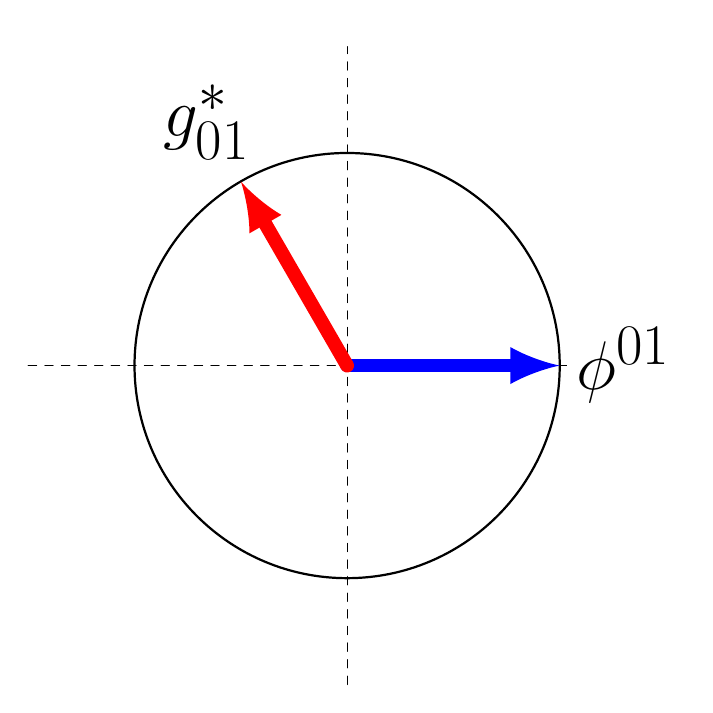
\begin{tikzpicture}[scale=2.7,cap=round,>=latex]
            % draw the coordinates
            \draw[dashed] (-1.5cm,0cm) -- (1.5cm,0cm) node[right,fill=white] {};
            \draw[dashed] (0cm,-1.5cm) -- (0cm,1.5cm) node[above,fill=white] {};
    
            % draw the unit circle
            \draw[thick] (0cm,0cm) circle(1cm);
    
            %phi01
            \draw[blue, ->, line width=5pt] (0cm,0cm) -- (0:1cm);

            %g01
            \draw[red, ->, line width=5pt] (0cm,0cm) -- (120:1cm);

            % text at the end
            \draw (0:1.3cm) node[fill=white, font=\Huge] {$\phi^{01}$};
            \draw (120:1.32cm) node[fill=white, font=\Huge] {$g_{01}^*$};
    
        \end{tikzpicture}}
        \text{\tiny $\boldsymbol{\alpha}$ = 00}
    \end{subfigure}%
    \begin{subfigure}[b]{0.105\textwidth}
        \centering
        \resizebox{\textwidth}{!}{
        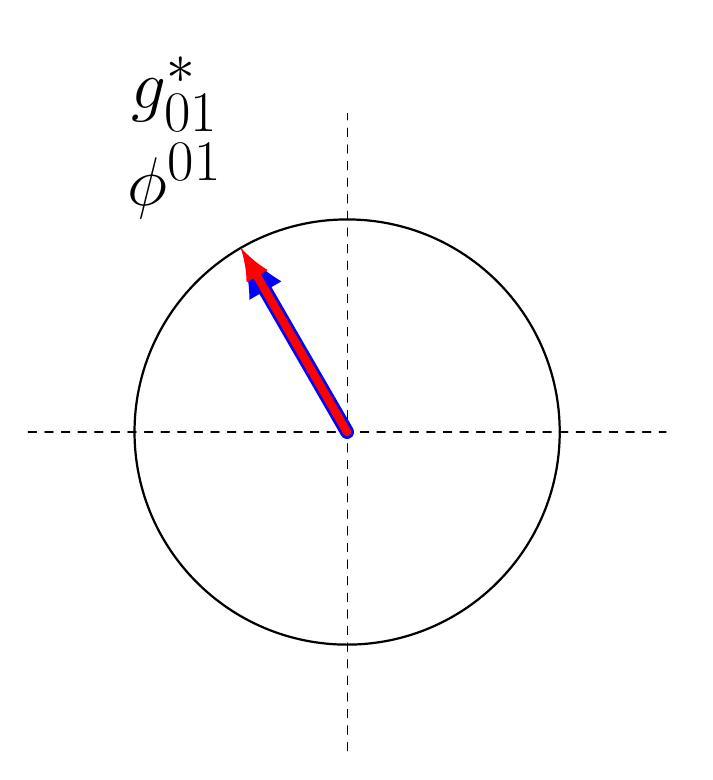
\begin{tikzpicture}[scale=2.7,cap=round,>=latex]
            % draw the coordinates
            \draw[dashed] (-1.5cm,0cm) -- (1.5cm,0cm) node[right,fill=white] {};
            \draw[dashed] (0cm,-1.5cm) -- (0cm,1.5cm) node[above,fill=white] {};
    
            % draw the unit circle
            \draw[thick] (0cm,0cm) circle(1cm);
    
            %phi01
            \draw[blue, ->, line width=5pt] (0cm,0cm) -- (120:1cm);

            %g01
            \draw[red, ->, line width=3pt] (0cm,0cm) -- (120:1cm);

            % text at the end
            \setlength\extrarowheight{5pt}
            \draw (120:1.62cm) node[fill=white, font=\Huge] {\begin{tabular}{c} $g_{01}^*$\\ $\phi^{01}$\end{tabular}};

        \end{tikzpicture}}
        \text{\tiny $\boldsymbol{\alpha}$ = 11}
    \end{subfigure}%
    \begin{subfigure}[b]{0.105\textwidth}
        \centering
        \resizebox{\textwidth}{!}{
        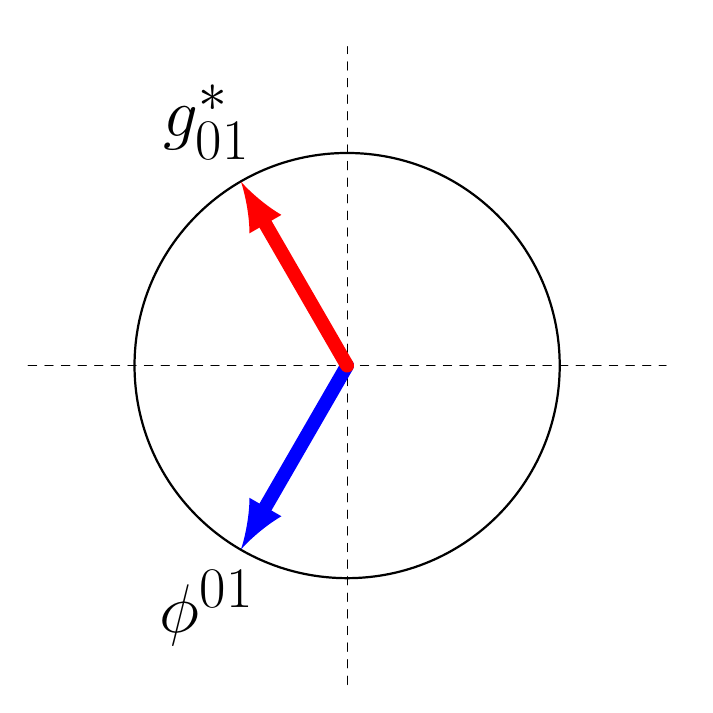
\begin{tikzpicture}[scale=2.7,cap=round,>=latex]
            % draw the coordinates
            \draw[dashed] (-1.5cm,0cm) -- (1.5cm,0cm) node[right,fill=white] {};
            \draw[dashed] (0cm,-1.5cm) -- (0cm,1.5cm) node[above,fill=white] {};
    
            % draw the unit circle
            \draw[thick] (0cm,0cm) circle(1cm);
    
            %phi01
            \draw[blue, ->, line width=5pt] (0cm,0cm) -- (240:1cm);

            %g01
            \draw[red, ->, line width=5pt] (0cm,0cm) -- (120:1cm);

            % text at the end
            \draw (240:1.32cm) node[fill=white, font=\Huge] {$\phi^{01}$};
            \draw (120:1.32cm) node[fill=white, font=\Huge] {$g_{01}^*$};

        \end{tikzpicture}}
        \text{\tiny $\boldsymbol{\alpha}$ = 22}
    \end{subfigure}
    \hfill
    \begin{subfigure}[b]{0.105\textwidth}
        \centering
        \resizebox{\textwidth}{!}{
        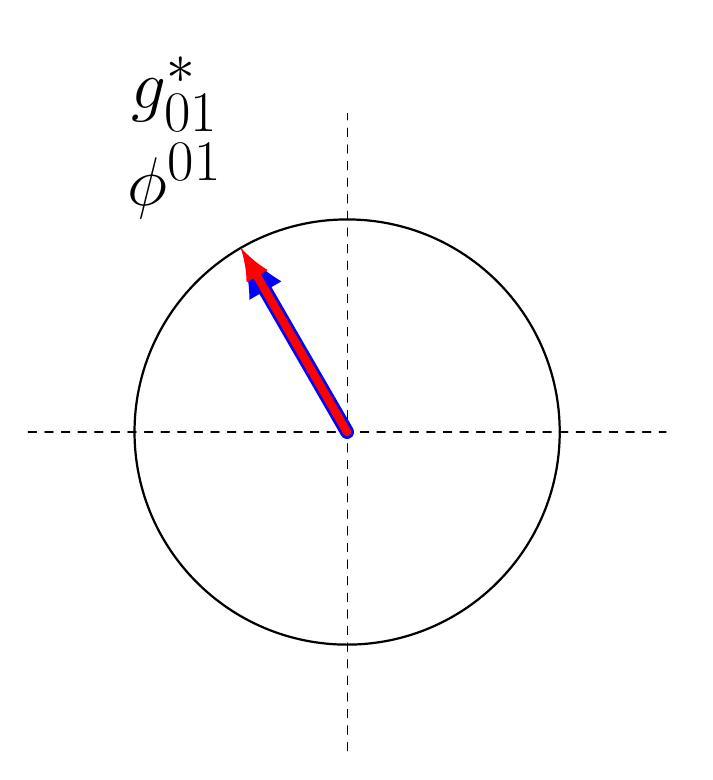
\begin{tikzpicture}[scale=2.7,cap=round,>=latex]
            % draw the coordinates
            \draw[dashed] (-1.5cm,0cm) -- (1.5cm,0cm) node[right,fill=white] {};
            \draw[dashed] (0cm,-1.5cm) -- (0cm,1.5cm) node[above,fill=white] {};
    
            % draw the unit circle
            \draw[thick] (0cm,0cm) circle(1cm);
    
            %phi01
            \draw[blue, ->, line width=5pt] (0cm,0cm) -- (120:1cm);

            %g01
            \draw[red, ->, line width=3pt] (0cm,0cm) -- (120:1cm);

            % text at the end
            \setlength\extrarowheight{5pt}
            \draw (120:1.62cm) node[fill=white, font=\Huge] {\begin{tabular}{c} $g_{01}^*$\\ $\phi^{01}$\end{tabular}};
    
        \end{tikzpicture}}
        \text{\tiny $\boldsymbol{\alpha}$ = 01}
    \end{subfigure}%
    \begin{subfigure}[b]{0.105\textwidth}
        \centering
        \resizebox{\textwidth}{!}{
        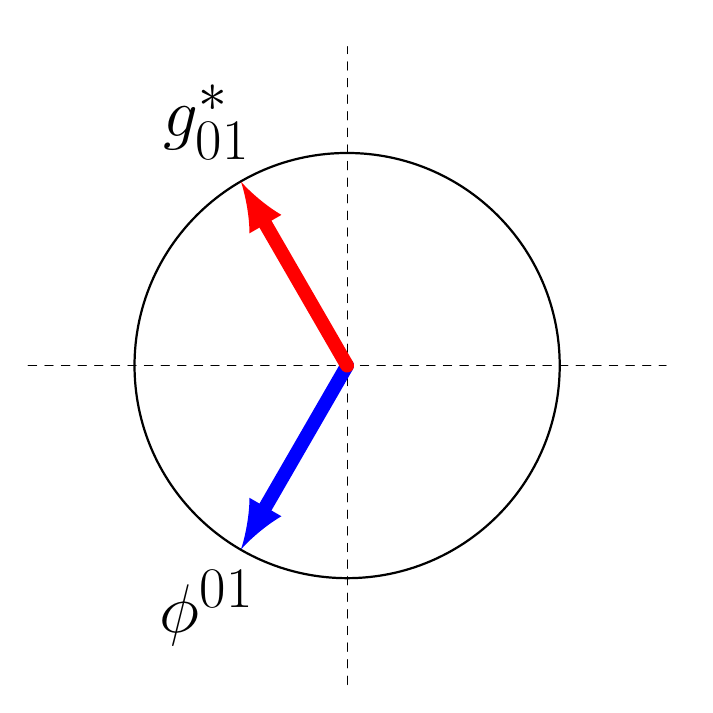
\begin{tikzpicture}[scale=2.7,cap=round,>=latex]
            % draw the coordinates
            \draw[dashed] (-1.5cm,0cm) -- (1.5cm,0cm) node[right,fill=white] {};
            \draw[dashed] (0cm,-1.5cm) -- (0cm,1.5cm) node[above,fill=white] {};
    
            % draw the unit circle
            \draw[thick] (0cm,0cm) circle(1cm);
    
            %phi01
            \draw[blue, ->, line width=5pt] (0cm,0cm) -- (240:1cm);

            %g01
            \draw[red, ->, line width=5pt] (0cm,0cm) -- (120:1cm);

            % text at the end
            \draw (240:1.32cm) node[fill=white, font=\Huge] {$\phi^{01}$};
            \draw (120:1.32cm) node[fill=white, font=\Huge] {$g_{01}^*$};

        \end{tikzpicture}}
        \text{\tiny $\boldsymbol{\alpha}$ = 12}
    \end{subfigure}%
    \begin{subfigure}[b]{0.105\textwidth}
        \centering
        \resizebox{\textwidth}{!}{
        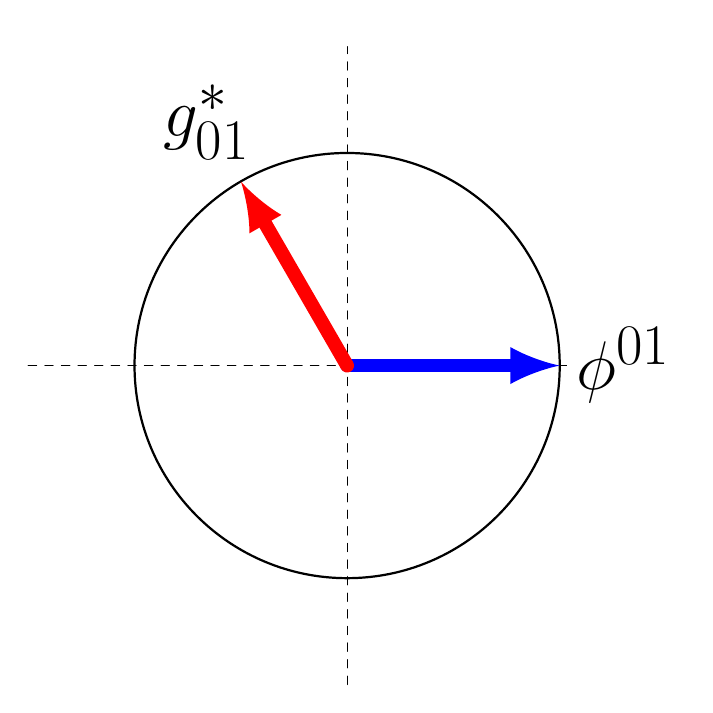
\begin{tikzpicture}[scale=2.7,cap=round,>=latex]
            % draw the coordinates
            \draw[dashed] (-1.5cm,0cm) -- (1.5cm,0cm) node[right,fill=white] {};
            \draw[dashed] (0cm,-1.5cm) -- (0cm,1.5cm) node[above,fill=white] {};
    
            % draw the unit circle
            \draw[thick] (0cm,0cm) circle(1cm);
    
            %phi01
            \draw[blue, ->, line width=5pt] (0cm,0cm) -- (0:1cm);

            %g01
            \draw[red, ->, line width=5pt] (0cm,0cm) -- (120:1cm);

            % text at the end
            \draw (0:1.3cm) node[fill=white, font=\Huge] {$\phi^{01}$};
            \draw (120:1.32cm) node[fill=white, font=\Huge] {$g_{01}^*$};
    
        \end{tikzpicture}}
        \text{\tiny $\boldsymbol{\alpha}$ = 20}
    \end{subfigure}
    \hfill
    \begin{subfigure}[b]{0.105\textwidth}
        \centering
        \resizebox{\textwidth}{!}{
        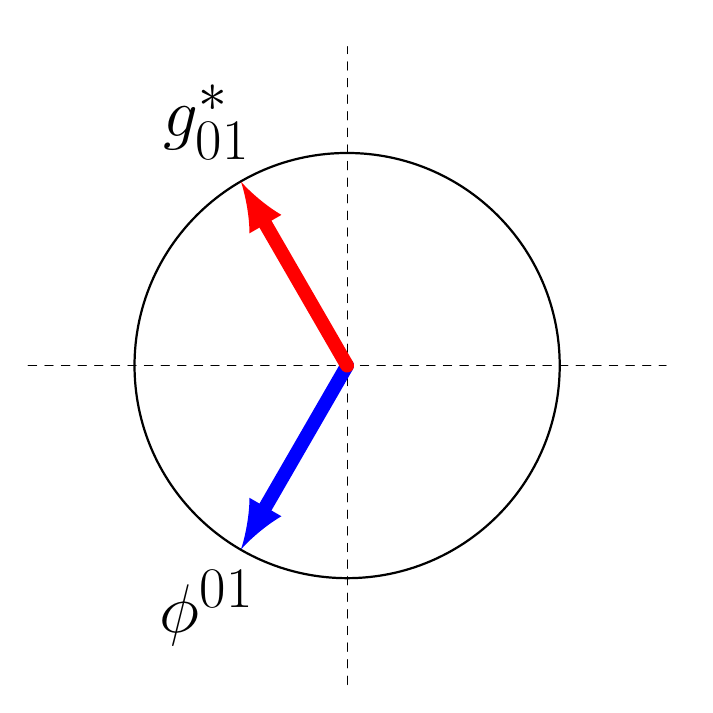
\begin{tikzpicture}[scale=2.7,cap=round,>=latex]
            % draw the coordinates
            \draw[dashed] (-1.5cm,0cm) -- (1.5cm,0cm) node[right,fill=white] {};
            \draw[dashed] (0cm,-1.5cm) -- (0cm,1.5cm) node[above,fill=white] {};
    
            % draw the unit circle
            \draw[thick] (0cm,0cm) circle(1cm);
    
            %phi01
            \draw[blue, ->, line width=5pt] (0cm,0cm) -- (240:1cm);

            %g01
            \draw[red, ->, line width=5pt] (0cm,0cm) -- (120:1cm);

            % text at the end
            \draw (240:1.32cm) node[fill=white, font=\Huge] {$\phi^{01}$};
            \draw (120:1.32cm) node[fill=white, font=\Huge] {$g_{01}^*$};

        \end{tikzpicture}}
        \text{\tiny $\boldsymbol{\alpha}$ = 02}
    \end{subfigure}%
    \begin{subfigure}[b]{0.105\textwidth}
        \centering
        \resizebox{\textwidth}{!}{
        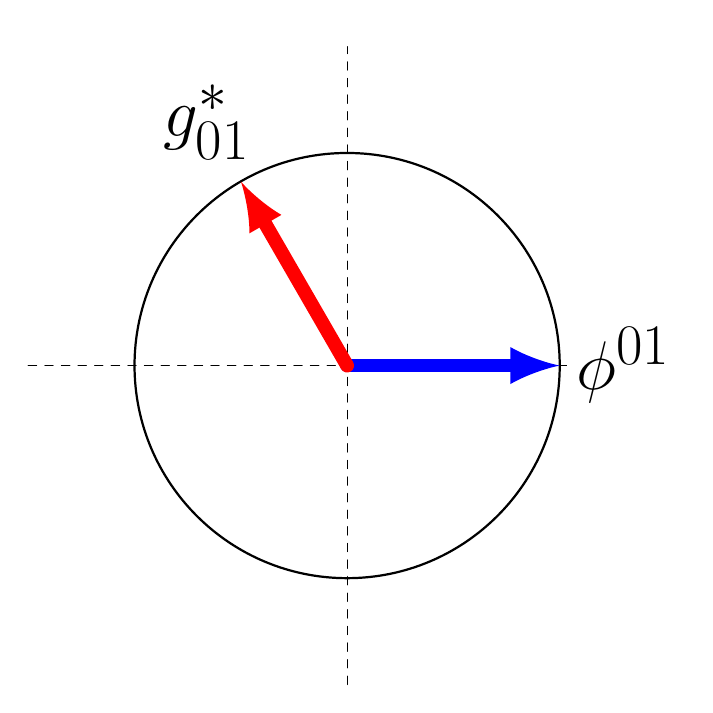
\begin{tikzpicture}[scale=2.7,cap=round,>=latex]
            % draw the coordinates
            \draw[dashed] (-1.5cm,0cm) -- (1.5cm,0cm) node[right,fill=white] {};
            \draw[dashed] (0cm,-1.5cm) -- (0cm,1.5cm) node[above,fill=white] {};
    
            % draw the unit circle
            \draw[thick] (0cm,0cm) circle(1cm);
    
            %phi01
            \draw[blue, ->, line width=5pt] (0cm,0cm) -- (0:1cm);

            %g01
            \draw[red, ->, line width=5pt] (0cm,0cm) -- (120:1cm);

            % text at the end
            \draw (0:1.3cm) node[fill=white, font=\Huge] {$\phi^{01}$};
            \draw (120:1.32cm) node[fill=white, font=\Huge] {$g_{01}^*$};
    
        \end{tikzpicture}}
        \text{\tiny $\boldsymbol{\alpha}$ = 10}
    \end{subfigure}%
    \begin{subfigure}[b]{0.105\textwidth}
        \centering
        \resizebox{\textwidth}{!}{
        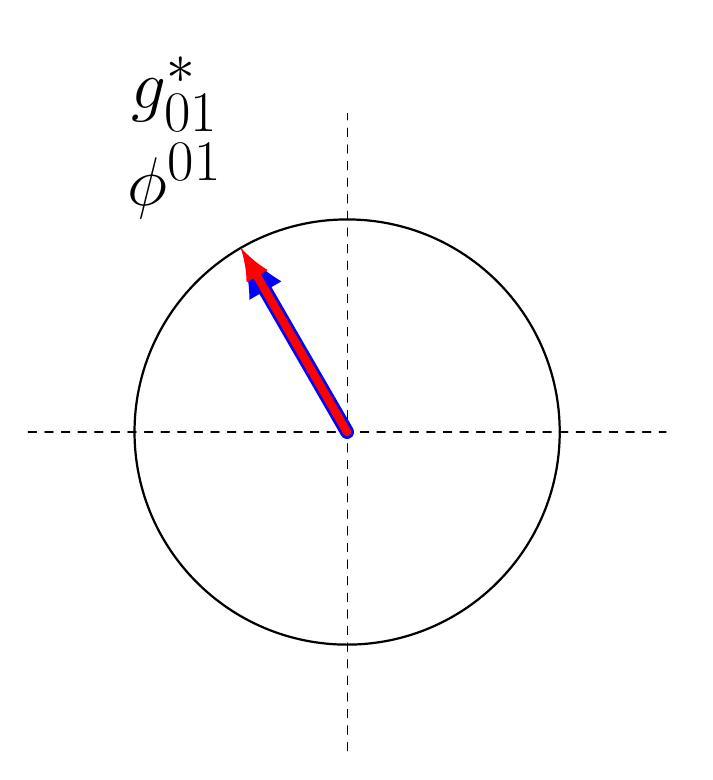
\begin{tikzpicture}[scale=2.7,cap=round,>=latex]
            % draw the coordinates
            \draw[dashed] (-1.5cm,0cm) -- (1.5cm,0cm) node[right,fill=white] {};
            \draw[dashed] (0cm,-1.5cm) -- (0cm,1.5cm) node[above,fill=white] {};
    
            % draw the unit circle
            \draw[thick] (0cm,0cm) circle(1cm);
    
            %phi01
            \draw[blue, ->, line width=5pt] (0cm,0cm) -- (120:1cm);

            %g01
            \draw[red, ->, line width=3pt] (0cm,0cm) -- (120:1cm);

            % text at the end
            \setlength\extrarowheight{5pt}
            \draw (120:1.62cm) node[fill=white, font=\Huge] {\begin{tabular}{c} $g_{01}^*$\\ $\phi^{01}$\end{tabular}};

        \end{tikzpicture}}
        \text{\tiny $\boldsymbol{\alpha}$ = 21}
    \end{subfigure}%
    \caption{Graphical representation of $S({\boldsymbol{\alpha}})$ of a 3-state,2-spin system with a first-order interaction, $\phi^{01}$ and $\phi^{01}$, and a second order interaction, $\phi^{12}$ and $\phi^{21}$. The parameters for the first-order interaction are chosen such that states where $\alpha_2 = 1$ are preferred and the parameters of the second-order interactions such that states for which  $\sum_{j \in \mu} \alpha_j \mu_j =  0\mod3$ are preferred.}
    \label{fig:s_case_2}
\end{figure}

\begin{table}[h]
    \centering
    \caption{Numerical values for S($\boldsymbol{\alpha}$) and P($\boldsymbol{\alpha}$) for a spin model with a first-order interaction, $\phi^{01}$ and $\phi^{01}$, and a second order interaction, $\phi^{12}$ and $\phi^{21}$.}
    \label{tab:case_2_num_values}
    \begin{subtable}{.3\textwidth}
        \centering
        \caption{r = 0.5}
        \begin{tabular}{ccc}
            \toprule
             $\boldsymbol{\alpha}$ & S($\boldsymbol{\alpha}$) & P($\boldsymbol{\alpha}$)\\
            \midrule
            00 & 0.5 & 0.107 \\
            01 & 0.5 & 0.107 \\
            02 & -1 & 0.024 \\
            10 & -1 & 0.024 \\
            11 & 2 & 0.478 \\
            12 & -1 & 0.024 \\
            20 & -1 & 0.024 \\
            21 & 0.5 & 0.107 \\
            22 & 0.5 & 0.107\\
          \bottomrule
        \end{tabular}
    \end{subtable}%
    \begin{subtable}{.3\textwidth}
        \centering
        \caption{r = 1}
        \begin{tabular}{ccc}
            \toprule
             $\boldsymbol{\alpha}$ & S($\boldsymbol{\alpha}$) & P($\boldsymbol{\alpha}$)\\
            \midrule
            00 & 1 & 0.041 \\
            01 & 1 & 0.041 \\
            02 & -2 & 0.002 \\
            10 & -2 & 0.002 \\
            11 & 4 & 0.827 \\
            12 & -2 & 0.002 \\
            20 & -2 & 0.002 \\
            21 & 1 & 0.041 \\
            22 & 1 & 0.041 \\
          \bottomrule
        \end{tabular}
    \end{subtable}%
    \begin{subtable}{.3\textwidth}
        \centering
        \caption{r = 2}
        \begin{tabular}{ccc}
            \toprule
             $\boldsymbol{\alpha}$ & S($\boldsymbol{\alpha}$) & P($\boldsymbol{\alpha}$)\\
            \midrule
            00 & 2 & 0.002 \\
            01 & 2 & 0.002 \\
            02 & -4 & 0.000 \\
            10 & -4 & 0.000 \\
            11 & 8 & 0.990 \\
            12 & -4 & 0.000 \\
            20 & -4 & 0.000 \\
            21 & 2 & 0.002 \\
            22 & 2 & 0.002 \\
          \bottomrule
        \end{tabular}
    \end{subtable}
\end{table}

\noindent
\textit{Case 3: Two second-order interactions}

\begin{itemize}
    \item $g_{11}$ = $r\left[\cos\left( \frac{4\pi}{3}\right) + i \sin\left( \frac{4\pi}{3}\right)\right]$
    \item $g_{22}$ = $r\left[\cos\left( \frac{4\pi}{3}\right) - i \sin\left( \frac{4\pi}{3}\right)\right]$
    \item $g_{12}$ = $r$
    \item $g_{21}$ = $r$
\end{itemize}

\begin{figure}[h!]
    \centering
    \begin{subfigure}[b]{0.33\textwidth}
        \centering
        \resizebox{\textwidth}{!}{
        \begin{tikzpicture}[scale=2.7,cap=round,>=latex]
            % draw the coordinates
            \draw[dashed] (-1.5cm,0cm) -- (1.5cm,0cm) node[right,fill=white] {};
            \draw[dashed] (0cm,-1.5cm) -- (0cm,1.5cm) node[above,fill=white] {};
    
            % draw the unit circle
            \draw[thick] (0cm,0cm) circle(1cm);
    
            %phi12
            \draw[blue, ->, ultra thick] (0cm,0cm) -- (0:1cm);

            %g12
            \draw[red, ->, thick] (0cm,0cm) -- (0:1cm);

            %projection
            \filldraw[black] (0:1cm) circle(0.6pt);

            % text at the end
            \draw (0:1.25cm) node[fill=white] {\begin{tabular}{c} $g_{12}^*$\\$\phi^{12}$\end{tabular}};
    
            % draw the horizontal and vertical coordinates
            \draw (1.45cm,0cm)  node[above=1pt] {$\Re$}
                (0cm,1.4cm)  node[fill=white] {$\Im$};
        \end{tikzpicture}}
    \end{subfigure}%
    \begin{subfigure}[b]{0.33\textwidth}
        \centering
        \resizebox{\textwidth}{!}{
        \begin{tikzpicture}[scale=2.7,cap=round,>=latex]
            % draw the coordinates
            \draw[dashed] (-1.5cm,0cm) -- (1.5cm,0cm) node[right,fill=white] {};
            \draw[dashed] (0cm,-1.5cm) -- (0cm,1.5cm) node[above,fill=white] {};
    
            % draw the unit circle
            \draw[thick] (0cm,0cm) circle(1cm);
    
            %phi12
            \draw[blue, ->, ultra thick] (0cm,0cm) -- (240:1cm);

            %g12
            \draw[red, ->, ultra thick] (0cm,0cm) -- (0:1cm);

            %projection
            \draw[dashdotted] (0:1cm) -- (60:.5cm);
            \filldraw[black] (60:.5cm) circle(0.6pt);

            % text at the end
            \draw (240:1.3cm) node[fill=white] {\begin{tabular}{c} $\phi^{12}$\end{tabular}};
            \draw (0:1.15cm) node[fill=white] {$g_{12}^*$};
        
            % draw the horizontal and vertical coordinates
            \draw (1.4cm,0cm)  node[above=1pt] {$\Re$}
                (0cm,1.4cm)  node[fill=white] {$\Im$};
        \end{tikzpicture}}
    \end{subfigure}%
    \begin{subfigure}[b]{0.33\textwidth}
        \centering
        \resizebox{\textwidth}{!}{
        \begin{tikzpicture}[scale=2.7,cap=round,>=latex]
            % draw the coordinates
            \draw[dashed] (-1.5cm,0cm) -- (1.5cm,0cm) node[right,fill=white] {};
            \draw[dashed] (0cm,-1.5cm) -- (0cm,1.5cm) node[above,fill=white] {};
    
            % draw the unit circle
            \draw[thick] (0cm,0cm) circle(1cm);
        
            %phi12
            \draw[blue, ->, ultra thick] (0cm,0cm) -- (120:1cm);

            %g12
            \draw[red, ->, ultra thick] (0cm,0cm) -- (0:1cm);

            %projection
            \draw[dashdotted] (0:1cm) -- (300:.5cm);
            \filldraw[black] (300:.5cm) circle(0.6pt);

            % text at the end
            \draw (120:1.3cm) node[fill=white] {\begin{tabular}{c} $\phi^{12}$\end{tabular}};
            \draw (0:1.15cm) node[fill=white] {$g_{12}^*$};
        
            % draw the horizontal and vertical coordinates
            \draw (1.5cm,0cm)  node[above=1pt] {$\Re$}
                (0cm,1.4cm)  node[fill=white] {$\Im$};
        \end{tikzpicture}}
    \end{subfigure}
    \begin{subfigure}[b]{0.105\textwidth}
        \centering
        \resizebox{\textwidth}{!}{
        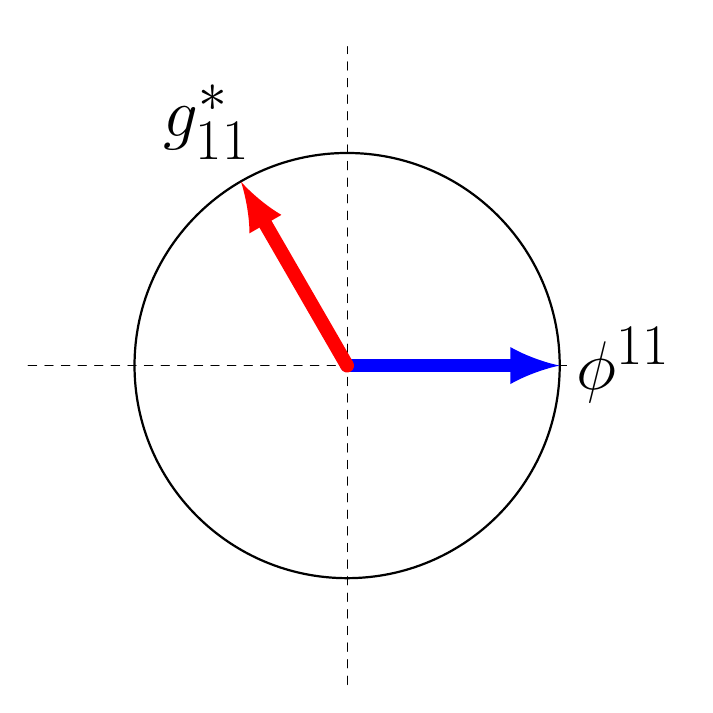
\begin{tikzpicture}[scale=2.7,cap=round,>=latex]
            % draw the coordinates
            \draw[dashed] (-1.5cm,0cm) -- (1.5cm,0cm) node[right,fill=white] {};
            \draw[dashed] (0cm,-1.5cm) -- (0cm,1.5cm) node[above,fill=white] {};
    
            % draw the unit circle
            \draw[thick] (0cm,0cm) circle(1cm);
    
            %phi11
            \draw[blue, ->, line width=5pt] (0cm,0cm) -- (0:1cm);

            %g11
            \draw[red, ->, line width=5pt] (0cm,0cm) -- (120:1cm);

            % text at the end
            \draw (0:1.3cm) node[fill=white, font=\Huge] {$\phi^{11}$};
            \draw (120:1.32cm) node[fill=white, font=\Huge] {$g_{11}^*$};
    
        \end{tikzpicture}}
        \text{\tiny $\boldsymbol{\alpha}$ = 00}
    \end{subfigure}%
    \begin{subfigure}[b]{0.105\textwidth}
        \centering
        \resizebox{\textwidth}{!}{
        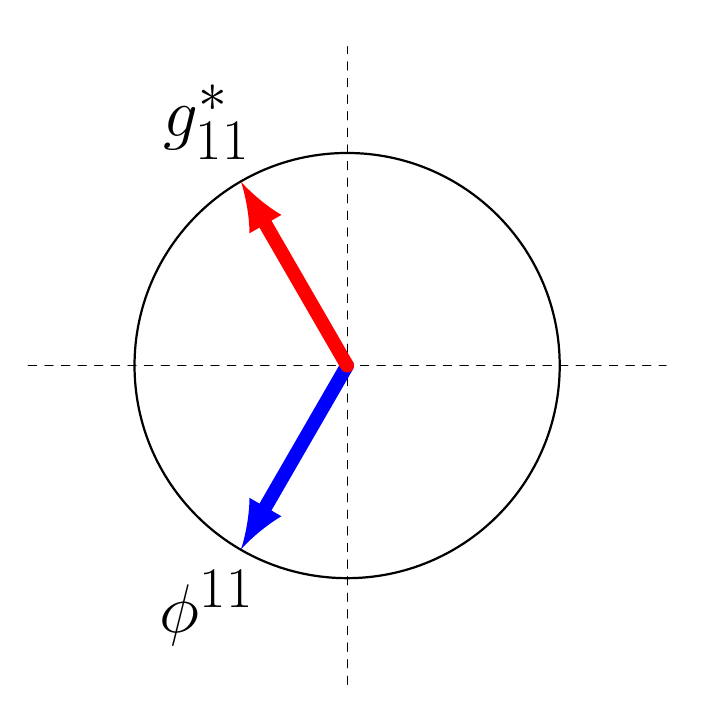
\begin{tikzpicture}[scale=2.7,cap=round,>=latex]
            % draw the coordinates
            \draw[dashed] (-1.5cm,0cm) -- (1.5cm,0cm) node[right,fill=white] {};
            \draw[dashed] (0cm,-1.5cm) -- (0cm,1.5cm) node[above,fill=white] {};
    
            % draw the unit circle
            \draw[thick] (0cm,0cm) circle(1cm);
    
            %phi11
            \draw[blue, ->, line width=5pt] (0cm,0cm) -- (240:1cm);

            %g11
            \draw[red, ->, line width=5pt] (0cm,0cm) -- (120:1cm);

            % text at the end
            \draw (240:1.32cm) node[fill=white, font=\Huge] {$\phi^{11}$};
            \draw (120:1.32cm) node[fill=white, font=\Huge] {$g_{11}^*$};
    
        \end{tikzpicture}}
        \text{\tiny $\boldsymbol{\alpha}$ = 11}
    \end{subfigure}%
    \begin{subfigure}[b]{0.105\textwidth}
        \centering
        \resizebox{\textwidth}{!}{
        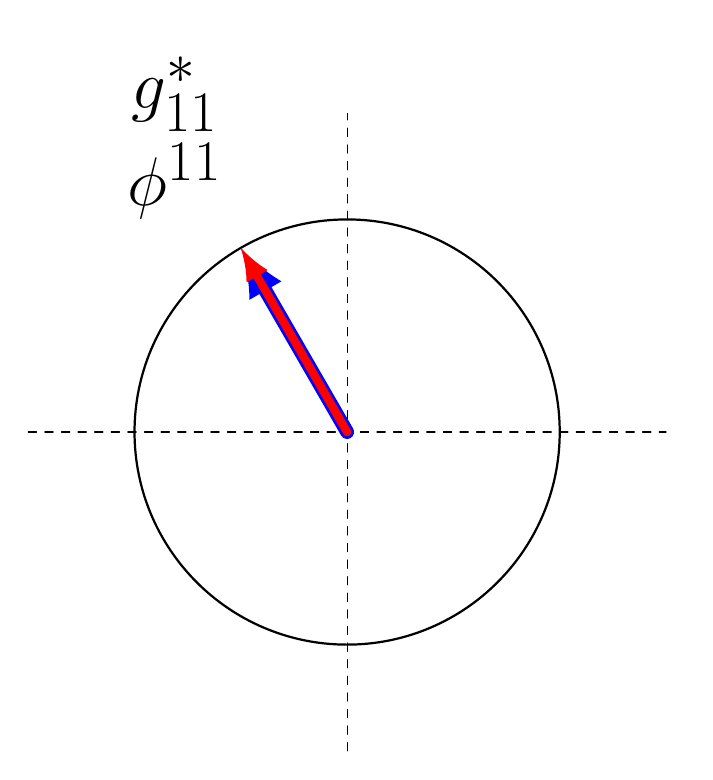
\begin{tikzpicture}[scale=2.7,cap=round,>=latex]
            % draw the coordinates
            \draw[dashed] (-1.5cm,0cm) -- (1.5cm,0cm) node[right,fill=white] {};
            \draw[dashed] (0cm,-1.5cm) -- (0cm,1.5cm) node[above,fill=white] {};
    
            % draw the unit circle
            \draw[thick] (0cm,0cm) circle(1cm);
    
            %phi11
            \draw[blue, ->, line width=5pt] (0cm,0cm) -- (120:1cm);

            %g11
            \draw[red, ->, line width=3pt] (0cm,0cm) -- (120:1cm);

            % text at the end
            \setlength\extrarowheight{5pt}
            \draw (120:1.62cm) node[fill=white, font=\Huge] {\begin{tabular}{c} $g_{11}^*$\\ $\phi^{11}$\end{tabular}};

        \end{tikzpicture}}
        \text{\tiny $\boldsymbol{\alpha}$ = 22}
    \end{subfigure}
    \hfill
    \begin{subfigure}[b]{0.105\textwidth}
        \centering
        \resizebox{\textwidth}{!}{
        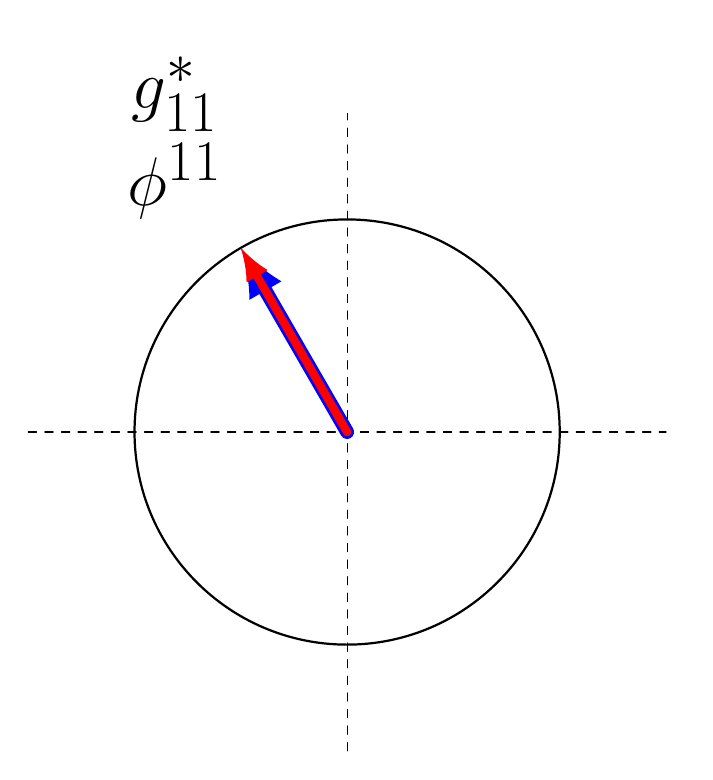
\begin{tikzpicture}[scale=2.7,cap=round,>=latex]
            % draw the coordinates
            \draw[dashed] (-1.5cm,0cm) -- (1.5cm,0cm) node[right,fill=white] {};
            \draw[dashed] (0cm,-1.5cm) -- (0cm,1.5cm) node[above,fill=white] {};
    
            % draw the unit circle
            \draw[thick] (0cm,0cm) circle(1cm);
    
            %phi11
            \draw[blue, ->, line width=5pt] (0cm,0cm) -- (120:1cm);

            %g11
            \draw[red, ->, line width=3pt] (0cm,0cm) -- (120:1cm);

            % text at the end
            \setlength\extrarowheight{5pt}
            \draw (120:1.62cm) node[fill=white, font=\Huge] {\begin{tabular}{c} $g_{11}^*$\\ $\phi^{11}$\end{tabular}};

        \end{tikzpicture}}
        \text{\tiny $\boldsymbol{\alpha}$ = 01}
    \end{subfigure}%
    \begin{subfigure}[b]{0.105\textwidth}
        \centering
        \resizebox{\textwidth}{!}{
        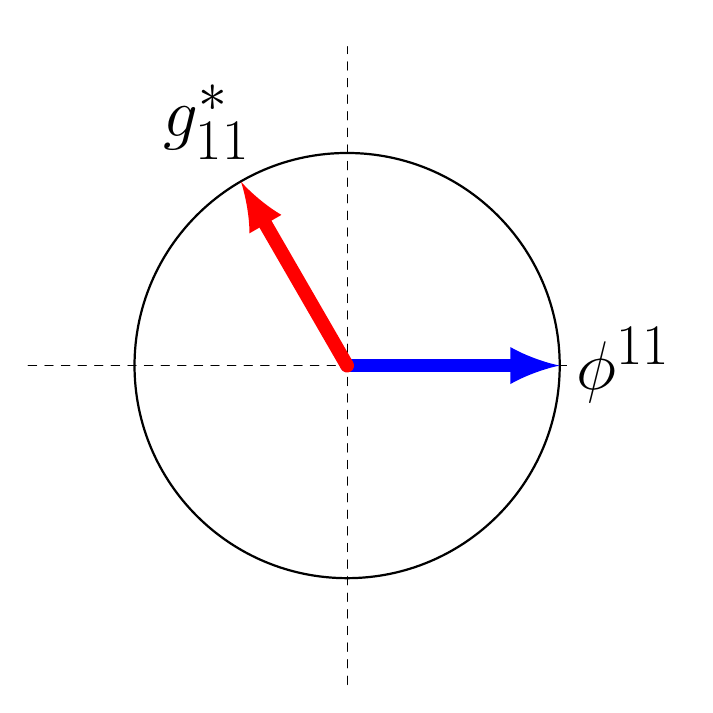
\begin{tikzpicture}[scale=2.7,cap=round,>=latex]
            % draw the coordinates
            \draw[dashed] (-1.5cm,0cm) -- (1.5cm,0cm) node[right,fill=white] {};
            \draw[dashed] (0cm,-1.5cm) -- (0cm,1.5cm) node[above,fill=white] {};
    
            % draw the unit circle
            \draw[thick] (0cm,0cm) circle(1cm);
    
            %phi11
            \draw[blue, ->, line width=5pt] (0cm,0cm) -- (0:1cm);

            %g11
            \draw[red, ->, line width=5pt] (0cm,0cm) -- (120:1cm);

            % text at the end
            \draw (0:1.3cm) node[fill=white, font=\Huge] {$\phi^{11}$};
            \draw (120:1.32cm) node[fill=white, font=\Huge] {$g_{11}^*$};
    
        \end{tikzpicture}}
        \text{\tiny $\boldsymbol{\alpha}$ = 12}
    \end{subfigure}%
    \begin{subfigure}[b]{0.105\textwidth}
        \centering
        \resizebox{\textwidth}{!}{
        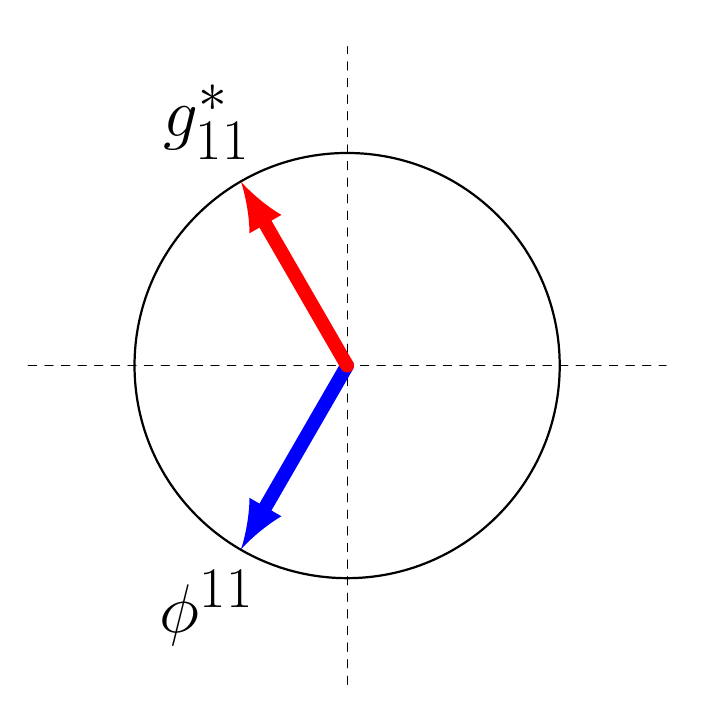
\begin{tikzpicture}[scale=2.7,cap=round,>=latex]
            % draw the coordinates
            \draw[dashed] (-1.5cm,0cm) -- (1.5cm,0cm) node[right,fill=white] {};
            \draw[dashed] (0cm,-1.5cm) -- (0cm,1.5cm) node[above,fill=white] {};
    
            % draw the unit circle
            \draw[thick] (0cm,0cm) circle(1cm);
    
            %phi11
            \draw[blue, ->, line width=5pt] (0cm,0cm) -- (240:1cm);

            %g11
            \draw[red, ->, line width=5pt] (0cm,0cm) -- (120:1cm);

            % text at the end
            \draw (240:1.32cm) node[fill=white, font=\Huge] {$\phi^{11}$};
            \draw (120:1.32cm) node[fill=white, font=\Huge] {$g_{11}^*$};
    
        \end{tikzpicture}}
        \text{\tiny $\boldsymbol{\alpha}$ = 20}
    \end{subfigure}
    \hfill
    \begin{subfigure}[b]{0.105\textwidth}
        \centering
        \resizebox{\textwidth}{!}{
        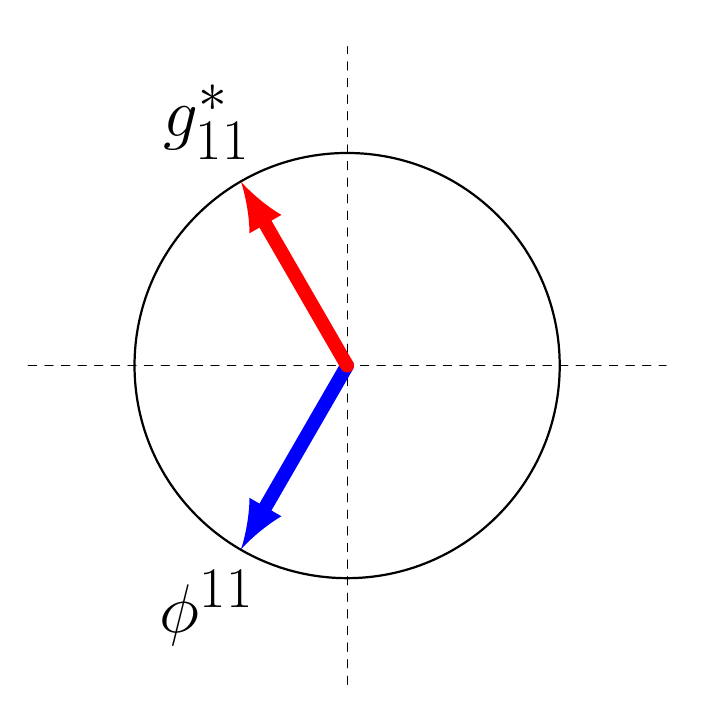
\begin{tikzpicture}[scale=2.7,cap=round,>=latex]
            % draw the coordinates
            \draw[dashed] (-1.5cm,0cm) -- (1.5cm,0cm) node[right,fill=white] {};
            \draw[dashed] (0cm,-1.5cm) -- (0cm,1.5cm) node[above,fill=white] {};
    
            % draw the unit circle
            \draw[thick] (0cm,0cm) circle(1cm);
    
            %phi11
            \draw[blue, ->, line width=5pt] (0cm,0cm) -- (240:1cm);

            %g11
            \draw[red, ->, line width=5pt] (0cm,0cm) -- (120:1cm);

            % text at the end
            \draw (240:1.32cm) node[fill=white, font=\Huge] {$\phi^{11}$};
            \draw (120:1.32cm) node[fill=white, font=\Huge] {$g_{11}^*$};
    
        \end{tikzpicture}}
        \text{\tiny $\boldsymbol{\alpha}$ = 02}
    \end{subfigure}%
    \begin{subfigure}[b]{0.105\textwidth}
        \centering
        \resizebox{\textwidth}{!}{
        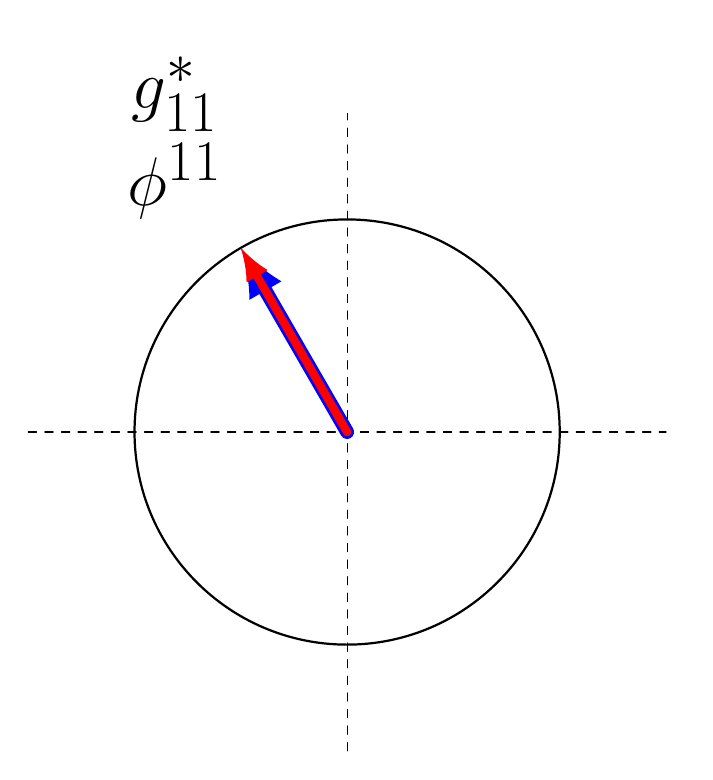
\begin{tikzpicture}[scale=2.7,cap=round,>=latex]
            % draw the coordinates
            \draw[dashed] (-1.5cm,0cm) -- (1.5cm,0cm) node[right,fill=white] {};
            \draw[dashed] (0cm,-1.5cm) -- (0cm,1.5cm) node[above,fill=white] {};
    
            % draw the unit circle
            \draw[thick] (0cm,0cm) circle(1cm);
    
            %phi11
            \draw[blue, ->, line width=5pt] (0cm,0cm) -- (120:1cm);

            %g11
            \draw[red, ->, line width=3pt] (0cm,0cm) -- (120:1cm);

            % text at the end
            \setlength\extrarowheight{5pt}
            \draw (120:1.62cm) node[fill=white, font=\Huge] {\begin{tabular}{c} $g_{11}^*$\\ $\phi^{11}$\end{tabular}};

        \end{tikzpicture}}
        \text{\tiny $\boldsymbol{\alpha}$ = 10}
    \end{subfigure}%
    \begin{subfigure}[b]{0.105\textwidth}
        \centering
        \resizebox{\textwidth}{!}{
        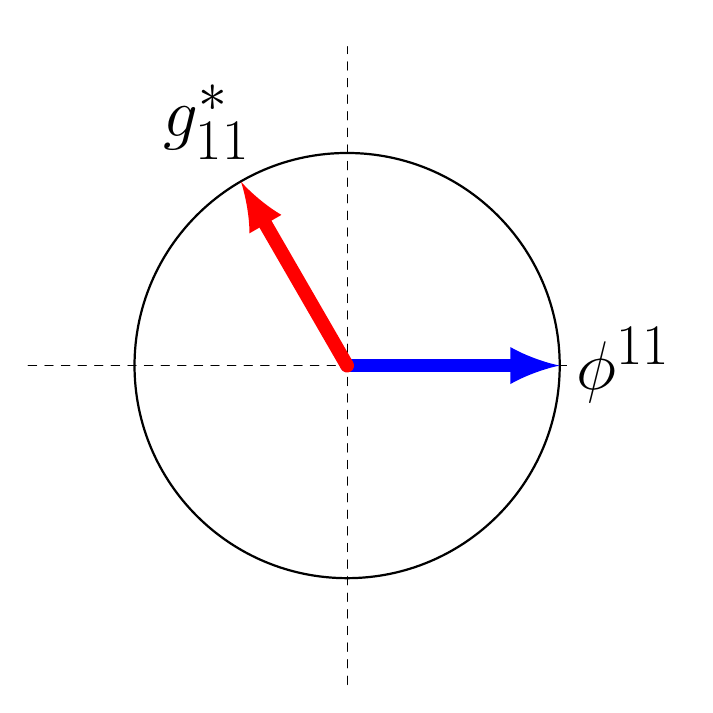
\begin{tikzpicture}[scale=2.7,cap=round,>=latex]
            % draw the coordinates
            \draw[dashed] (-1.5cm,0cm) -- (1.5cm,0cm) node[right,fill=white] {};
            \draw[dashed] (0cm,-1.5cm) -- (0cm,1.5cm) node[above,fill=white] {};
    
            % draw the unit circle
            \draw[thick] (0cm,0cm) circle(1cm);
    
            %phi11
            \draw[blue, ->, line width=5pt] (0cm,0cm) -- (0:1cm);

            %g11
            \draw[red, ->, line width=5pt] (0cm,0cm) -- (120:1cm);

            % text at the end
            \draw (0:1.3cm) node[fill=white, font=\Huge] {$\phi^{11}$};
            \draw (120:1.32cm) node[fill=white, font=\Huge] {$g_{11}^*$};
    
        \end{tikzpicture}}
        \text{\tiny $\boldsymbol{\alpha}$ = 21}
    \end{subfigure}%
    \caption{Graphical representation of $S({\boldsymbol{\alpha}})$ of a 3-state,2-spin system with two second order interactions. 
    The parameter $g_{12}$ is chosen such that states for which  $\sum_{j \in \mu} \alpha_j \mu_j =  0\mod3$ are preferred and the parameter $g_{11}$ is chosen such that states for which  $\sum_{j \in \mu} \alpha_j \mu_j =  1\mod3$ are preferred.}
    \label{fig:s_case_3}
\end{figure}

\begin{table}[h]
    \centering
    \caption{Numerical values for S($\boldsymbol{\alpha}$) and P($\boldsymbol{\alpha}$) for a spin model with two second order interactions.}
    \label{tab:case_2_num_values}
    \begin{subtable}{.3\textwidth}
        \centering
        \caption{r = 0.5}
        \begin{tabular}{ccc}
            \toprule
             $\boldsymbol{\alpha}$ & S($\boldsymbol{\alpha}$) & P($\boldsymbol{\alpha}$)\\
            \midrule
            00 & 0.5 & 0.107 \\
            01 & 0.5 & 0.107 \\
            02 & -1 & 0.024 \\
            10 & -1 & 0.024 \\
            11 & 2 & 0.478 \\
            12 & -1 & 0.024 \\
            20 & -1 & 0.024 \\
            21 & 0.5 & 0.107 \\
            22 & 0.5 & 0.107\\
          \bottomrule
        \end{tabular}
    \end{subtable}%
    \begin{subtable}{.3\textwidth}
        \centering
        \caption{r = 1}
        \begin{tabular}{ccc}
            \toprule
             $\boldsymbol{\alpha}$ & S($\boldsymbol{\alpha}$) & P($\boldsymbol{\alpha}$)\\
            \midrule
            00 & 1 & 0.041 \\
            01 & 1 & 0.041 \\
            02 & -2 & 0.002 \\
            10 & -2 & 0.002 \\
            11 & 4 & 0.827 \\
            12 & -2 & 0.002 \\
            20 & -2 & 0.002 \\
            21 & 1 & 0.041 \\
            22 & 1 & 0.041 \\
          \bottomrule
        \end{tabular}
    \end{subtable}%
    \begin{subtable}{.3\textwidth}
        \centering
        \caption{r = 2}
        \begin{tabular}{ccc}
            \toprule
             $\boldsymbol{\alpha}$ & S($\boldsymbol{\alpha}$) & P($\boldsymbol{\alpha}$)\\
            \midrule
            00 & 2 & 0.002 \\
            01 & 2 & 0.002 \\
            02 & -4 & 0.000 \\
            10 & -4 & 0.000 \\
            11 & 8 & 0.990 \\
            12 & -4 & 0.000 \\
            20 & -4 & 0.000 \\
            21 & 2 & 0.002 \\
            22 & 2 & 0.002 \\
          \bottomrule
        \end{tabular}
    \end{subtable}
\end{table}
\clearpage
\subsection{Model parameters in polar coordinates}\label{sec:polar_coord}

An alternative is to write the model parameters in polar coordinates,

\begin{equation}
    g_{\boldsymbol{\mu}} = r_{\boldsymbol{\mu}} e^{i \theta_{\boldsymbol{\mu}}}.
\end{equation}

\noindent
Then, the constraints are

\begin{equation}
    \begin{cases}
        r_{-\boldsymbol{\mu}} = r_{\boldsymbol{\mu}}\\
        \theta_{-\boldsymbol{\mu}} = -\theta_{\boldsymbol{\mu}}
    \end{cases}
    .
\end{equation}

\noindent
The function, $S(\alpha)$ of all three states can be expressed as

\begin{align*}
    S(\alpha=0) &= r_1 e^{i \theta_1} \phi^1(\alpha=0) + r_2 e^{i \theta_2} \phi^2(\alpha=0),\\
    S(\alpha=1) &= r_1 e^{i \theta_1} \phi^1(\alpha=1) + r_2 e^{i \theta_2} \phi^2(\alpha=1),\\
    S(\alpha=2) &= r_1 e^{i \theta_1} \phi^1(\alpha=2) + r_2 e^{i \theta_2} \phi^2(\alpha=2).
\end{align*}

\noindent
Plugging in the values for the spin operators and using the constraints gives,

\begin{align*}
    S(\alpha=0) &= r_1 e^{i \theta_1} + r_2 e^{i \theta_2},\\
    &= r_1 e^{i \theta_1} + r_1 e^{-i \theta_1}, \\
    &= r_1 \left[ \cos\left( \theta_1 \right) + i \sin\left( \theta_1 \right) + \cos\left( \theta_1 \right) - i \sin\left( \theta_1 \right) \right],\\
    &= 2r_1 \cos\left( \theta_1 \right),\\
    S(\alpha=1) &= r_1 e^{i \theta_1} e^{\frac{2\pi i}{3}} + r_2 e^{i \theta_2} e^{\frac{4\pi i}{3}},\\
    &= r_1 e^{i\left( \frac{2\pi}{3} + \theta_1 \right)} + r_2 e^{-i \left(\frac{2\pi}{3} - \theta_2 \right)},\\
    &= r_1 e^{i\left( \frac{2\pi}{3} + \theta_1 \right)} + r_1 e^{-i \left(\frac{2\pi}{3} + \theta_1 \right)},\\
    &= r_1 \left[ \cos\left( \frac{2\pi}{3} + \theta_1 \right) + i \sin \left( \frac{2\pi}{3} + \theta_1 \right) + \cos\left( \frac{2\pi}{3} + \theta_1 \right) - i \sin \left( \frac{2\pi}{3} + \theta_1 \right) \right],\\
    &= 2 r_1 \cos\left( \frac{2\pi}{3} + \theta_1 \right),\\
    S(\alpha=2) &= r_1 e^{i \theta_1} e^{\frac{4\pi i}{3}} + r_2 e^{i \theta_2} e^{\frac{2\pi i}{3}},\\
    &= r_1 e^{i\left( \frac{4\pi}{3} + \theta_1 \right)} + r_2 e^{-i \left(\frac{4\pi}{3} - \theta_2 \right)},\\
    &= r_1 e^{i\left( \frac{4\pi}{3} + \theta_1 \right)} + r_1 e^{-i \left(\frac{4\pi}{3} + \theta_1 \right)},\\
    &= r_1 \left[ \cos\left( \frac{4\pi}{3} + \theta_1 \right) + i \sin \left( \frac{4\pi}{3} + \theta_1 \right) + \cos\left( \frac{4\pi}{3} + \theta_1 \right) - i \sin \left( \frac{4\pi}{3} + \theta_1 \right) \right],\\
    &= 2 r_1 \cos\left( \frac{4\pi}{3} + \theta_1 \right).
\end{align*}

\noindent 
From these expressions, we can see that $S(\alpha=0)$ is maximized when $\theta_1$ is a multiple of $2\pi$. $S(\alpha=1)$ is maximized when $\frac{2\pi}{3} + \theta_1$ is a multiple of $2\pi$ or equivalent when $\theta_1$ is equal to $-\frac{2\pi}{3}$.
$S(\alpha=2)$ is maximized when $\frac{4\pi}{3} + \theta_1$ is a multiple of $2\pi$ or equivalent when $\theta_1$ is equal to $\frac{-4\pi}{3}$.
In general, $S(\alpha)$ and thus the probability of state $\alpha$ is maximally increased by a pair of conjugate spin operators when the complex conjugate of the parameters are aligned with the spin operators applied on the state $\alpha$.

\noindent
In Figure \ref{fig:s_alpha}, a graphical representation of $S({\alpha})$ is shown for a 3-state,1-spin system where the complex conjugate of $g_1$ aligns mostly with $\phi^1(\alpha=1)$.
Due to the constraints on the parameters, the complex conjugate of $g_2$ aligns mostly with $\phi^2(\alpha=1)$.
Figure \ref{fig:s_alpha_1} shows that this alignment results in a large positive real contribution to $S(\alpha = 1)$ of both $g_1 \phi^1(\alpha=1)$ and $g_2 \phi^2(\alpha=1)$. 
Note that the complex contributions of $g_1 \phi^1(\alpha=1)$ and $g_2 \phi^2(\alpha=1)$ cancel each other, which makes $S(\alpha=1)$ a real value.
In Figure \ref{fig:s_alpha_2}, the same thing is shown for $S(\alpha=2)$. Because the action of the spin operator on the state is different, both spin operators will have a negative real contribution to $S(\alpha=2)$.
Again, the complex contributions cancel each other due to the constraints on the model parameters.

\begin{figure}[h]
    \centering
    \begin{subfigure}[b]{0.5\textwidth}
        \centering
        \resizebox{\textwidth}{!}{
        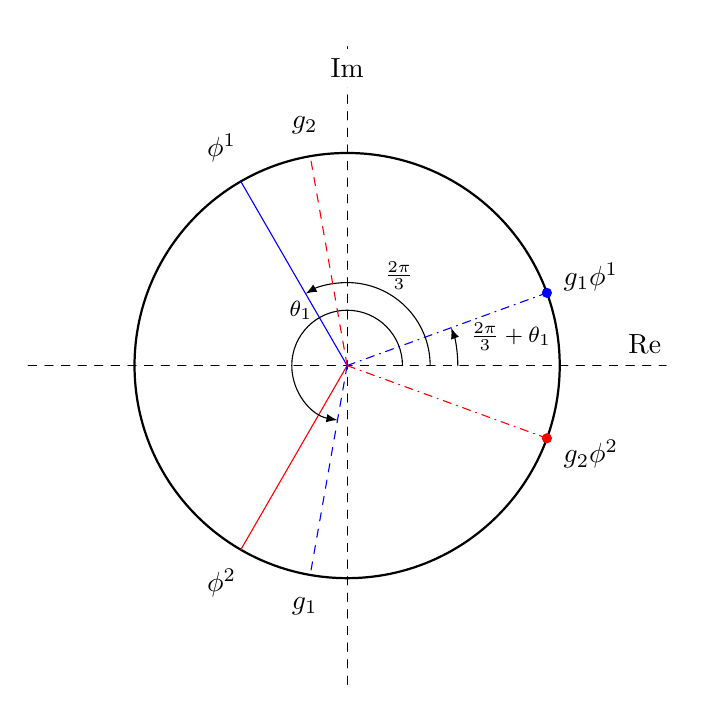
\begin{tikzpicture}[scale=2.7,cap=round,>=latex]
            %Origin
            \coordinate (O) at (0,0);
            %Coordinate (1,0)
            \coordinate (X) at (1,0);
            % draw the coordinates
            \draw[dashed] (-1.5cm,0cm) -- (1.5cm,0cm) node[right,fill=white] {};
            \draw[dashed] (0cm,-1.5cm) -- (0cm,1.5cm) node[above,fill=white] {};
    
            % draw the unit circle
            \draw[thick] (0cm,0cm) circle(1cm);
    
            %line for alpha = one state
            \draw[blue] (0cm,0cm) -- (120:1cm);
            % text at the end
            \draw (120:1.18cm) node[fill=white] {$\phi^1$};
            %draw angle
            \coordinate (phi1) at (120:1cm);
            \draw pic[->,"\footnotesize $\frac{2\pi}{3}$",draw=black,angle radius=30,angle eccentricity=1.25] {angle=X--O--phi1};
    
            %line for alpha = two state
            \draw[red] (0cm,0cm) -- (240:1cm);
            % text at the end
            \draw (240:1.18cm) node[fill=white] {$\phi^2$};
    
            %g1
            \draw[dashed, blue] (0cm,0cm) -- (260:1cm);
            % text at the end
            \draw (260:1.15cm) node[fill=white] {$g_1$};
            % draw angle
            \coordinate (G1) at (260:1cm);
            \draw pic[->,"\footnotesize $\theta_1$",draw=black,angle radius=20,angle eccentricity=1.3] {angle=X--O--G1};
    
            %g2
            \draw[dashed, red] (0cm,0cm) -- (100:1cm);
            % text at the end
            \draw (100:1.15cm) node[fill=white] {$g_2$};
    
            %g1 phi1
            \draw[dashdotted, blue] (0cm,0cm) -- (20:1cm);
            % dot at end point
            \filldraw[blue] (20:1cm) circle(0.6pt);
            % text at the end
            \draw (20:1.22cm) node[fill=white] {$g_1 \phi^1$};
            %draw angle
            \coordinate (G1_PHI1) at (20:1cm);
            \draw pic[->,"\footnotesize $\frac{2\pi}{3} +\theta_1$",draw=black,angle radius=40,angle eccentricity=1.5] {angle=X--O--G1_PHI1};
    
            %g2 phi2
            \draw[dashdotted, red] (0cm,0cm) -- (340:1cm);
            % dot at end point
            \filldraw[red] (340:1cm) circle(0.6pt);
            % text at the end
            \draw (340:1.22cm) node[fill=white] {$g_2 \phi^2$};
    
            % draw the horizontal and vertical coordinates
            \draw (1.4cm,0cm)  node[above=1pt] {$\Re$}
                (0cm,1.4cm)  node[fill=white] {$\Im$};
        \end{tikzpicture}}
        \caption{$S(\alpha = 1)$}\label{fig:s_alpha_1}
    \end{subfigure}%
    \begin{subfigure}[b]{0.5\textwidth}
        \centering
        \resizebox{\textwidth}{!}{
        \begin{tikzpicture}[scale=2.7,cap=round,>=latex]
            % draw the coordinates
            \draw[dashed] (-1.5cm,0cm) -- (1.5cm,0cm) node[right,fill=white] {};
            \draw[dashed] (0cm,-1.5cm) -- (0cm,1.5cm) node[above,fill=white] {};
    
            % draw the unit circle
            \draw[thick] (0cm,0cm) circle(1cm);

            %line for alpha = one state
            \draw[blue] (0cm,0cm) -- (240:1cm);
            % text at the end
            \draw (240:1.18cm) node[fill=white] {$\phi^1$};
    
            %line for alpha = two state
            \draw[red] (0cm,0cm) -- (120:1cm);
            % text at the end
            \draw (120:1.18cm) node[fill=white] {$\phi^2$};
    
            %g1
            \draw[dashed, blue] (0cm,0cm) -- (260:1cm);
            % text at the end
            \draw (260:1.15cm) node[fill=white] {$g_1$};
    
            %g2
            \draw[dashed, red] (0cm,0cm) -- (100:1cm);
            % text at the end
            \draw (100:1.15cm) node[fill=white] {$g_2$};
    
            %g1 phi1
            \draw[dashdotted, blue] (0cm,0cm) -- (140:1cm);
            % dot at end point
            \filldraw[blue] (140:1cm) circle(0.6pt);
            % text at the end
            \draw (140:1.22cm) node[fill=white] {$g_1 \phi^1$};
    
            %g2 phi2
            \draw[dashdotted, red] (0cm,0cm) -- (220:1cm);
            % dot at end point
            \filldraw[red] (220:1cm) circle(0.6pt);
            % text at the end
            \draw (220:1.22cm) node[fill=white] {$g_2 \phi^2$};

    
            % draw the horizontal and vertical coordinates
            \draw (1.4cm,0cm)  node[above=1pt] {$\Re$}
                (0cm,1.4cm)  node[fill=white] {$\Im$};
        \end{tikzpicture}}
        \caption{$S(\alpha = 2)$}\label{fig:s_alpha_2}
    \end{subfigure}
    \caption{Graphical representation of $S({\alpha})$ of a 3-state,1-spin system. The parameters $g_1$ and $g_2$ are chosen such that $g_1$ slightly deviates from the complex conjugate of $\phi^1(\alpha=1)$. The dots indicate the contributions to $S(\alpha)$.}
    \label{fig:s_alpha}
\end{figure}



%\printbibliography
%-------------------------------------------------------------------------------
%	REFERENCES
%-------------------------------------------------------------------------------

%-------------------------------------------------------------------------------
%	BIJLAGEN 
%-------------------------------------------------------------------------------



%-------------------------------------------------------------------------------
\end{document}


